\documentclass[a4paper,10pt,twoside]{report}
\usepackage[left=2cm,right=2cm,top=2cm,bottom=3cm]{geometry}

\usepackage{listings}
\usepackage{color}

\usepackage{xcolor}
\usepackage{colortbl}
 
\definecolor{codegreen}{rgb}{0,0.6,0}
\definecolor{codegray}{rgb}{0.5,0.5,0.5}
\definecolor{codepurple}{rgb}{0.58,0,0.82}
\definecolor{backcolour}{rgb}{0.95,0.95,0.92}

\newcommand{\mc}[2]{\multicolumn{#1}{c}{#2}}
\definecolor{Gray}{gray}{0.85}
\definecolor{LightCyan}{rgb}{0.88,1,1}
 
\lstdefinestyle{mystyle}{
    backgroundcolor=\color{backcolour},   
    commentstyle=\color{codegreen},
    keywordstyle=\color{magenta},
    numberstyle=\tiny\color{codegray},
    stringstyle=\color{codepurple},
    basicstyle=\footnotesize,
    breakatwhitespace=false,         
    breaklines=true,                 
    captionpos=b,                    
    keepspaces=true,                 
    numbers=left,                    
    numbersep=5pt,                  
    showspaces=false,                
    showstringspaces=false,
    showtabs=false,                  
    tabsize=2
}
 
\lstset{style=mystyle}

\lstdefinelanguage{Swift}{
  keywords={associatedtype, class, deinit, enum, extension, func, import, init, inout, internal, let, operator, private, protocol, public, static, struct, subscript, typealias, var, break, case, continue, default, defer, do, else, fallthrough, for, guard, if, in, repeat, return, switch, where, while, as, catch, dynamicType, false, is, nil, rethrows, super, self, Self, throw, throws, true, try, associativity, convenience, dynamic, didSet, final, get, infix, indirect, lazy, left, mutating, none, nonmutating, optional, override, postfix, precedence, prefix, Protocol, required, right, set, Type, unowned, weak, willSet},
  ndkeywords={class, export, boolean, throw, implements, import, this},
  sensitive=false,
  comment=[l]{//},
  morecomment=[s]{/*}{*/},
  morestring=[b]',
  morestring=[b]"
}

\usepackage{graphicx}
\usepackage{verbatim}
\usepackage{latexsym}
\usepackage{mathchars}
\usepackage{setspace}
\usepackage{tabularx} % in the preamble
\setlength{\parskip}{\medskipamount}  % a little space before a \par
\setlength{\parindent}{0pt}	      % don't indent first lines of paragraphs
\makeatletter
\def\chapapp2{Chapter}

\def\appendix{\par
 \setcounter{chapter}{0}
 \setcounter{section}{0}
 \def\chapapp2{Appendix}
 \def\@chapapp{Appendix}
 \def\thechapter{\Alph{chapter}}}

\def\ps@uheadings{\let\@mkboth\markboth
% modifications
\def\@oddhead{\protect\underline{\protect\makebox[\textwidth][l]
		{\sl\rightmark\hfill\rm\thepage}}}
\def\@oddfoot{}
\def\@evenfoot{}
\def\@evenhead{\protect\underline{\protect\makebox[\textwidth][l]
		{\rm\thepage\hfill\sl\leftmark}}}
% end of modifications
\def\chaptermark##1{\markboth {\ifnum \c@secnumdepth >\m@ne
 \chapapp2\ \thechapter. \ \fi ##1}{}}%
\def\sectionmark##1{\markright {\ifnum \c@secnumdepth >\z@
   \thesection. \ \fi ##1}}}
\makeatother
%%From: marcel@cs.caltech.edu (Marcel van der Goot)
%%Newsgroups: comp.text.tex
%%Subject: illegal modification of boxit.sty
%%Date: 28 Feb 92 01:10:02 GMT
%%Organization: California Institute of Technology (CS dept)
%%Nntp-Posting-Host: andromeda.cs.caltech.edu
%%
%%
%%Quite some time ago I posted a file boxit.sty; maybe it made it
%%to some archives, although I don't recall submitting it. It defines
%%	\begin{boxit}
%%	...
%%	\end{boxit}
%%to draw a box around `...', where the `...' can contain other
%%environments (e.g., a verbatim environment). Unfortunately, it had
%%a problem: it did not work if you used it in paragraph mode, i.e., it
%%only worked if there was an empty line in front of \begin{boxit}.
%%Luckily, that is easily corrected.
%%
%%HOWEVER, apparently someone noticed the problem, tried to correct it,
%%and then distributed this modified version. That would be fine with me,
%%except that:
%%1. There was no note in the file about this modification, it only has my
%%   name in it.
%%2. The modification is wrong: now it only works if there is *no* empty
%%   line in front of \begin{boxit}. In my opinion this bug is worse than
%%   the original one.
%%
%%In particular, the author of this modification tried to force an empty
%%line by inserting a `\\' in the definition of \Beginboxit. If you have
%%a version of boxit.sty with a `\\', please delete it. If you have my
%%old version of boxit.sty, please also delete it. Below is an improved
%%version.
%%
%%Thanks to Joe Armstrong for drawing my attention to the bug and to the
%%illegal version.
%%
%%                                          Marcel van der Goot
%% .---------------------------------------------------------------
%% | Blauw de viooltjes,                    marcel@cs.caltech.edu
%% |    Rood zijn de rozen;
%% | Een rijm kan gezet
%% |    Met plaksel en dozen.
%% |


% boxit.sty
% version: 27 Feb 1992
%
% Defines a boxit environment, which draws lines around its contents.
% Usage:
%   \begin{boxit}
%	... (text you want to be boxed, can contain other environments)
%   \end{boxit}
%
% The width of the box is the width of the contents.
% The boxit* environment behaves the same, except that the box will be
% at least as wide as a normal paragraph.
%
% The reason for writing it this way (rather than with the \boxit#1 macro
% from the TeXbook), is that now you can box verbatim text, as in
%   \begin{boxit}
%   \begin{verbatim}
%   this better come out in boxed verbatim mode ...
%   \end{verbatim}
%   \end{boxit}
%
%						Marcel van der Goot
%						marcel@cs.caltech.edu
%

\def\Beginboxit
   {\par
    \vbox\bgroup
	   \hrule
	   \hbox\bgroup
		  \vrule \kern1.2pt %
		  \vbox\bgroup\kern1.2pt
   }

\def\Endboxit{%
			      \kern1.2pt
		       \egroup
		  \kern1.2pt\vrule
		\egroup
	   \hrule
	 \egroup
   }	

\newenvironment{boxit}{\Beginboxit}{\Endboxit}
\newenvironment{boxit*}{\Beginboxit\hbox to\hsize{}}{\Endboxit}
\pagestyle{empty}

\setlength{\parskip}{2ex plus 0.5ex minus 0.2ex}
\setlength{\parindent}{0pt}

\makeatletter  %to avoid error messages generated by "\@". Makes Latex treat "@" like a letter

\linespread{1.5}
\def\submitdate#1{\gdef\@submitdate{#1}}

\def\maketitle{
  \begin{titlepage}{
    %\linespread{1.5}
    \Large Dublin Institute of Technology \\
    %\linebreak
    Department of Computing
    \rm
    \vskip 3in
    \Large \bf \@title \par
  }
  \vskip 0.3in
  \par
  {\Large \@author}
  \linebreak
  Student number: C13720705
  \linebreak
  \linebreak
  Supervisor: Edina Hatunic Webster
  \linebreak
  Second Reader: Susan McKeever
  \vskip 4in
  \par
  Submitted in part fulfilment of the requirements for the degree of 
  \linebreak
  Computer Science, \@submitdate
  \vfil
  \end{titlepage}
}

\def\titlepage{
  \newpage
  \centering
  \linespread{1}
  \normalsize
  \vbox to \vsize\bgroup\vbox to 9in\bgroup
}
\def\endtitlepage{
  \par
  \kern 0pt
  \egroup
  \vss
  \egroup
  \cleardoublepage
}

\def\abstract{
  \begin{center}{
    \large\bf Abstract}
  \end{center}
  \small
  %\def\baselinestretch{1.5}
  \linespread{1.5}
  \normalsize
}
\def\endabstract{
  \par
}

\newenvironment{acknowledgements}{
  \begin{center}{
    \large \bf Acknowledgements}
  \end{center}
  \small
  \linespread{1.5}
  \normalsize
}{\cleardoublepage}
\def\endacknowledgements{
  \par
}

\newenvironment{Declaration}{
  \newpage
  \begin{center}{
    \large \bf Declaration}
  \end{center}
  \small
  \linespread{1.5}
  \normalsize
}{\cleardoublepage}
\def\enddeclaration{
  \par
}

\def\preface{
    \pagenumbering{roman}
    \pagestyle{plain}
    \doublespacing
}

\def\body{
    \cleardoublepage    
    \pagestyle{uheadings}
    \tableofcontents
    \pagestyle{plain}
    \cleardoublepage
    \pagestyle{uheadings}
    \listoftables
    \pagestyle{plain}
    \pagestyle{uheadings}
    \listoffigures
    \pagestyle{plain}
    \lstlistoflistings
    \pagestyle{plain}
    \pagestyle{uheadings}
    \pagenumbering{arabic}
    \doublespacing
}

\makeatother
\usepackage{minted}

\usepackage{makecell}
\renewcommand\theadalign{cb}
\renewcommand\theadfont{\bfseries}
\renewcommand\theadgape{\Gape[4pt]}
\renewcommand\cellgape{\Gape[4pt]}

\newcommand{\ipc}{{\sf ipc}}

\newcommand{\Prob}{\bbbp}
\newcommand{\Real}{\bbbr}
\newcommand{\real}{\Real}
\newcommand{\Int}{\bbbz}
\newcommand{\Nat}{\bbbn}

\newcommand{\NN}{{\sf I\kern-0.14emN}}   % Natural numbers
\newcommand{\ZZ}{{\sf Z\kern-0.45emZ}}   % Integers
\newcommand{\QQQ}{{\sf C\kern-0.48emQ}}   % Rational numbers
\newcommand{\RR}{{\sf I\kern-0.14emR}}   % Real numbers
\newcommand{\KK}{{\cal K}}
\newcommand{\OO}{{\cal O}}
\newcommand{\AAA}{{\bf A}}
\newcommand{\HH}{{\bf H}}
\newcommand{\II}{{\bf I}}
\newcommand{\LL}{{\bf L}}
\newcommand{\PP}{{\bf P}}
\newcommand{\PPprime}{{\bf P'}}
\newcommand{\QQ}{{\bf Q}}
\newcommand{\UU}{{\bf U}}
\newcommand{\UUprime}{{\bf U'}}
\newcommand{\zzero}{{\bf 0}}
\newcommand{\ppi}{\mbox{\boldmath $\pi$}}
\newcommand{\aalph}{\mbox{\boldmath $\alpha$}}
\newcommand{\bb}{{\bf b}}
\newcommand{\ee}{{\bf e}}
\newcommand{\mmu}{\mbox{\boldmath $\mu$}}
\newcommand{\vv}{{\bf v}}
\newcommand{\xx}{{\bf x}}
\newcommand{\yy}{{\bf y}}
\newcommand{\zz}{{\bf z}}
\newcommand{\oomeg}{\mbox{\boldmath $\omega$}}
\newcommand{\res}{{\bf res}}
\newcommand{\cchi}{{\mbox{\raisebox{.4ex}{$\chi$}}}}
%\newcommand{\cchi}{{\cal X}}
%\newcommand{\cchi}{\mbox{\Large $\chi$}}

% Logical operators and symbols
\newcommand{\imply}{\Rightarrow}
\newcommand{\bimply}{\Leftrightarrow}
\newcommand{\union}{\cup}
\newcommand{\intersect}{\cap}
\newcommand{\boolor}{\vee}
\newcommand{\booland}{\wedge}
\newcommand{\boolimply}{\imply}
\newcommand{\boolbimply}{\bimply}
\newcommand{\boolnot}{\neg}
\newcommand{\boolsat}{\!\models}
\newcommand{\boolnsat}{\!\not\models}


\newcommand{\op}[1]{\mathrm{#1}}
\newcommand{\s}[1]{\ensuremath{\mathcal #1}}

% Properly styled differentiation and integration operators
\newcommand{\diff}[1]{\mathrm{\frac{d}{d\mathit{#1}}}}
\newcommand{\diffII}[1]{\mathrm{\frac{d^2}{d\mathit{#1}^2}}}
\newcommand{\intg}[4]{\int_{#3}^{#4} #1 \, \mathrm{d}#2}
\newcommand{\intgd}[4]{\int\!\!\!\!\int_{#4} #1 \, \mathrm{d}#2 \, \mathrm{d}#3}

% Large () brackets on different lines of an eqnarray environment
\newcommand{\Leftbrace}[1]{\left(\raisebox{0mm}[#1][#1]{}\right.}
\newcommand{\Rightbrace}[1]{\left.\raisebox{0mm}[#1][#1]{}\right)}

% Funky symobols for footnotes
\newcommand{\symbolfootnote}{\renewcommand{\thefootnote}{\fnsymbol{footnote}}}
% now add \symbolfootnote to the beginning of the document...

\newcommand{\normallinespacing}{\renewcommand{\baselinestretch}{1.5} \normalsize}
\newcommand{\mediumlinespacing}{\renewcommand{\baselinestretch}{1.2} \normalsize}
\newcommand{\narrowlinespacing}{\renewcommand{\baselinestretch}{1.0} \normalsize}
\newcommand{\bump}{\noalign{\vspace*{\doublerulesep}}}
\newcommand{\cell}{\multicolumn{1}{}{}}
\newcommand{\spann}{\mbox{span}}
\newcommand{\diagg}{\mbox{diag}}
\newcommand{\modd}{\mbox{mod}}
\newcommand{\minn}{\mbox{min}}
\newcommand{\andd}{\mbox{and}}
\newcommand{\forr}{\mbox{for}}
\newcommand{\EE}{\mbox{E}}

\newcommand{\deff}{\stackrel{\mathrm{def}}{=}}
\newcommand{\syncc}{~\stackrel{\textstyle \rhd\kern-0.57em\lhd}{\scriptstyle L}~}

\def\coop{\mbox{\large $\rhd\!\!\!\lhd$}}
\newcommand{\sync}[1]{\raisebox{-1.0ex}{$\;\stackrel{\coop}{\scriptscriptstyle
#1}\,$}}

\newtheorem{definition}{Definition}[chapter]
\newtheorem{theorem}{Theorem}[chapter]

\newcolumntype{L}[1]{>{\raggedright\let\newline\\\arraybackslash\hspace{0pt}}m{#1}}
\newcolumntype{C}[1]{>{\centering\let\newline\\\arraybackslash\hspace{0pt}}m{#1}}
\newcolumntype{R}[1]{>{\raggedleft\let\newline\\\arraybackslash\hspace{0pt}}m{#1}}

% \newcommand{\Figref}[1]{Figure~\ref{#1}}
% \newcommand{\fig}[3]{
%  \begin{figure}[!ht]
%  \begin{center}
%  \scalebox{#3}{\includegraphics{figs/#1.ps}}
%  \vspace{-0.1in}
%  \caption[ ]{\label{#1} #2}
%  \end{center}
%  \end{figure}
% }

% \newcommand{\figtwo}[8]{
%  \begin{figure}
%  \parbox[b]{#4 \textwidth}{
%  \begin{center}
%  \scalebox{#3}{\includegraphics{figs/#1.ps}}
%  \vspace{-0.1in}
%  \caption{\label{#1}#2}
%  \end{center}
%  }
%  \hfill
%  \parbox[b]{#8 \textwidth}{
%  \begin{center}
%  \scalebox{#7}{\includegraphics{figs/#5.ps}}
%  \vspace{-0.1in}
%  \caption{\label{#5}#6}
%  \end{center}
%  }
%  \end{figure}
% }


\begin{document}

\title{\LARGE {\bf Mobile Back-end as a Service iOS}\\
 \vspace*{6mm}
}

\author{Timothy Barnard}
\submitdate{4th April 2017}

\normallinespacing
\maketitle

\preface
\addcontentsline{toc}{chapter}{Abstract}

\begin{abstract}

Mobile applications are what we use everyday, they are part of our everyday life. Over the past number of years where mobile application development has boomed, so has the number of new developers wanting to build applications. This project due to time will only concentrate on iOS mobile development and with the new programming language Swift. Youtube channels have increased with the amount of tutorials for iOS development, but there still can be room for improvement. Some new and experience developers can be put off designing and creating a new application due to time and resources. Cloud services that govern the mobile industry are not cheap and easy to use, and this can be an obstacle for making mobile applications.

The aim of this project is help speed up development and testing, to be able to publish quicker, and to also provide a service that does not cost anything, that the developer has full control. The idea behind this will not only help in the development and testing parts, but also when the application is published. To be able to give the app a new look and feel without requiring a complete build and published, and to allow the end user more freedom with the design. This build will done along side Apples strict and fair guidelines to ensure its validity.

\end{abstract}
\clearpage

\addcontentsline{toc}{chapter}{Acknowledgements}

\begin{acknowledgements}

I would like to express my gratitude towards my supervisor, Edina Hatunic Webster for her continued help. Her guidance to keep me on tract for the deadline, and giving me continuous feedback.

I would also like to thank Susan McKeever for being my second reader, and for helping with getting outsourced developers to give me feedback on the project. This has helped me further with not only getting constructive feedback but also validating the project. 

The project would not be completed on time without the help of two mentors, and been a pleasure working along both of them.

I would like finally thank my family and friends for being there thought my college years.

\end{acknowledgements}
\cleardoublepage

\begin{Declaration}
Declaration


I hereby declare that the work described in this dissertation is, except where otherwise stated, entirely my own work and has not been submitted as an exercise for a degree at this or any other university.


Signed:

---------------------------------------------------

Timothy Barnard
4th April 2017

\end{Declaration}
\narrowlinespacing

\vspace*{4mm}

`Quote text here.'\\
\\
\emph{Guy Quoted}

\normallinespacing

\body
\chapter{Project Introduction}

\section{Overview}

What is Backend as a Service ? It is a way for developers to link their applications to backend cloud-based storage and services.Back-end as a service or BaaS is best described by a tech analyst who refers to it as "turn-on infrastructure" for mobile and web apps. Basically it's a cloud computing category that's comprised of companies that make it easier for developers to setup, use and operate a cloud backend for their mobile, tablet and web apps \cite{kinveywebsite}.  

\section{Project Objectives}
The aim of the this project is to develop a template for the development of mobile applications. This template is to help improve the development of modern mobile applications for new and experienced developers. This is achieved by providing services to help with the different phases of development. The project aim is to create a complete package that will enable new and experience developers speed up in the following areas:

\begin{enumerate}
  \item Development
  \item Testing 
  \item Production
\end{enumerate}

The project deliverables to aid with the three phases include the following:

\begin{enumerate}
  \item Dashboard
  
    The dashboard is a control panel that simplifies configuring applications. It also has data visualization to help improve the user experience when using the applications.
  \item Mobile Back-end as a Service
  
    This is a model for developers to link their applications to the backend cloud storage and application programming interfaces (API's) exposed to provide the communication with the list of services above.
  \item iOS Framework
  
    The services above need a way to communicate from back-end to the mobile apps. This is accomplish by providing a custom software development kits (SDKs).
\end{enumerate}

\section{Project Challenges}

The key challenge of the project was to find what developers functional requirements looking for when choosing a mobile backend as a service what current providers do not offer. This required setting up meetings with professional mobile developers and get their opinion on the project.

The big challenge faced was to find a way to enhance the developing stage of any application, giving more power to the developer when the application has been published. This lead to another challenge to see how far Apple would allow applications to be configured after published.

\section{Chapter Walk-through}

\paragraph{Chapter 2 Research}

This chapters discusses the alternative existing solutions to the problem. It also goes into the potential technologies that could be used in the project along with the resultant findings. The technologies discussed will be what web server to use, the programming language and what the dashboard be development in. This chapter will include surveys and out-sourced discussions with professional mobile developers.

\paragraph{Chapter 5 Architecture}

The architecture chapter will show the overview diagram of the complete project, along with diagrams of the individual services.

\paragraph{Chapter 4 Design}

This chapters goes into the design of the projects. What methodologies will be used?, and go into detail of the list of features already mentioned in project objectives section.

\paragraph{Chapter 5 Development}

This chapter will discuses the different deliverable in the project in order to achieve the project aim. It will contain detail description of the features that will be used to aid in mobile application development.

\paragraph{Chapter 6 Implementation}

Implementation chapters explains how to use different deliverables included in the project. Along with code snippets which show how to set up the system and use the SDK.

\paragraph{Chapter 7 Testing/Evaluation}

This chapter will give an overview of all testing carried out including test-driven approach and unit service testing. The evaluation section discusses the review given from the out-source professional developers. The review not only includes their feedback using the system but also their recommendations where to from here. 

\paragraph{Chapter 8 Conclusion}
The conclusion chapter contains a summary of the project overall and ends with a reflection of the project.

\paragraph{Chapter 9 Cases}
The conclusion chapter discusses the meetings and evaluations with out-sourced professional mobile app developers.
\chapter{Research}

\label{ch:background}

\section{Introduction}

The main focus of the project is to provide new and experienced mobile developers with three deliverables. The deliverables will bring something new to the table, a new way of developing applications. These deliverables are as follows:

\begin{itemize}
  \item Mobile Back-end as a Service
  \item Mobile framework (SDK)
  \item Dashboard
\end{itemize}

This chapter will not only cover the background research required for the deliverables, but also research from mobile developers and general mobile users. It will also cover the technologies required along with the current similar solutions.

\section{Background}

\subsection{Project deliverables}

\subsubsection{Mobile Back-end as a Service}

BaaS is an approach for providing mobile app developers a way to connect their application to back-end cloud storage and processing while also providing common features such as user management, push notifications, storage, and other  features that mobile users demand from their apps these days. The objective of any developer is to get their product finished and publish as quickly as possible. By providing a MBaaS to developers, it reduces time and resources needed to develop an app. As a research paper from Kinvey \cite{kinveywebsite} states these points regarding what BaaS delivers:

\begin{itemize}
  \item Efficiency Gains
    - Reducing overhead in all aspects of mobile app development, increasing efficiency at all stages of development
  \item Faster Times to Market
    - Reducing the obstacles to take a mobile app from idea to production and overhead with operations once in production
  \item App Delivery With Fewer Resources
    - BaaS supports development with fewer developers and supporting data and IT resources
  \item Optimize for Mobile and Tablets
    - BaaS providers have put a lot of time and resources into optimization of data and network for mobile apps, and reduce fragmentation problems across multiple platforms and devices.
  \item Secure and Scalable Infrastructure
    -  BaaS provides a bundled infrastructure that deals with scalability, security, performance and other operational headaches, leaving developers to do what they do best
  \item Stack of Common API resources 
    - BaaS brings common and essential 3rd party API resources into a single stack, preventing developers from having to go gather them separately
\end{itemize}

After reviewing why developers should use a MBaaS, the research paper goes on to discuss a pattern of building blocks being to emerge. These are the basic services that any MBaaS provider should be offering.

\begin{itemize}
  \item User Management
    - It all starts with a user, the ability for users to sign up and log in.
  \item Storage
    - a central location for all app data to be stored to connect all users together.
  \item Rest API
    - the link between the back-end services and client applications.
  \item Communication
    - feature such as push notifications to keep users connected live with other users.
\end{itemize}

In the technologies section will go into what web-server will be used along with programming language required. 

\subsubsection{Mobile framework}

Mobile frameworks helps with dealing with complex project such as integrating the MBaaS in apps. This is accomplish by using a dependency manager, which is a tool that manages all of the libraries in a meaningful and logical manner. By dependencies, its the libraries to make the application work with the MBaaS. There are a few of iOS dependency managers which can be used which will discussed in the technologies section.

\subsubsection{Dashboard}

\subsection{Mobile developers}

The key part of this project is to research from experienced developers, asking them in person and in forums. I have put up multiple questions in different forums regarding the functionality required for mobile Baas; What advantages and disadvantages do you find with current third party mobile back-end as a services?, What features do you want to be included in these services that you do not see at the moment? and Where do you see the future of third party services going, are they required or should mobile developers implement their own back-end? I have not been quite successful with these forums questions as most questions have to be problem specific but I have had some feedback.

I met with Trust5 \cite{trust5} and Tapadoo \cite{tapadoo}, two mobile software developing companies based in Dublin, Ireland to discuss my project proposal. The general feedback was positive, seeing the potential and powerful tool it could be. I had a working prototype iPad app  to demonstrate the remote configuration service as part of my project which updates a client mobile app interface which I will explain later. See appendix for the case study of each company.

\subsection{Mobile users}

Surveys were created to help get mobile users feedback using apps. The reason for this to be part for the research is that they are the end-user. They are the ones we want to keep happy, keep using our apps. The survey contained a number of questions which along with the results are as follows:

\subsubsection{1. Would you delete an app if it crashes?}

\begin{figure}[!h]
    \centering
    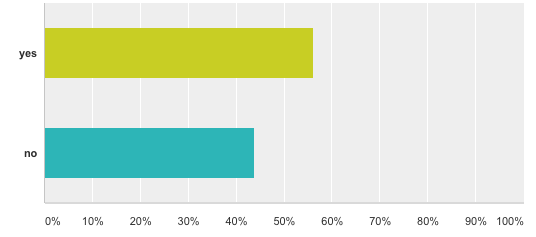
\includegraphics[width=100mm]{images/survey/crashes}
    \label{fig:label}
\end{figure}

\subsubsection{2. If you had a choice between two of the same type apps, Do you choose based on?}

\begin{figure}[!h]
    \centering
    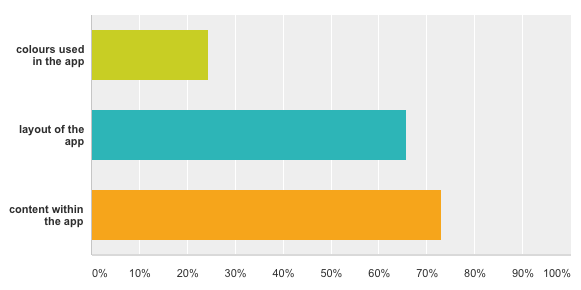
\includegraphics[width=100mm]{images/survey/choose}
    \label{fig:label}
\end{figure}

\subsubsection{3. How often do you like app updates?}

\begin{figure}[!h]
    \centering
    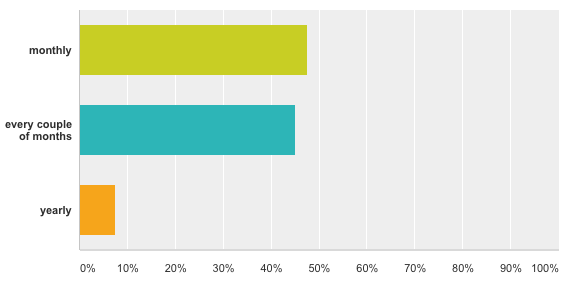
\includegraphics[width=100mm]{images/survey/time}
    \label{fig:label}
\end{figure}


\subsubsection{4. Would you prefer the user interface to be kept up to date and fresh more often?}

\begin{figure}[!h]
    \centering
    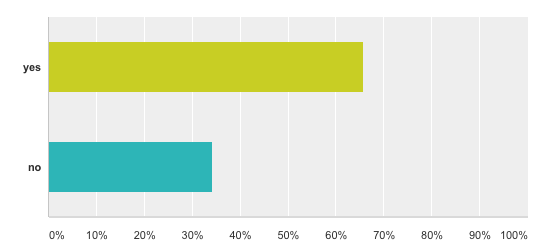
\includegraphics[width=100mm]{images/survey/updates}
    \label{fig:label}
\end{figure}

\subsubsection{5. Would you prefer being given the option for language choice (eg. English)?}

\begin{figure}[!h]
    \centering
    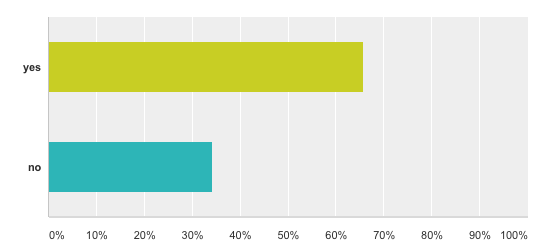
\includegraphics[width=100mm]{images/survey/language}
    \label{fig:label}
\end{figure}


\subsubsection{6. Do you mind apps collecting analytics in the background to help improve the app ? (not personal information)}

\begin{figure}[!h]
    \centering
    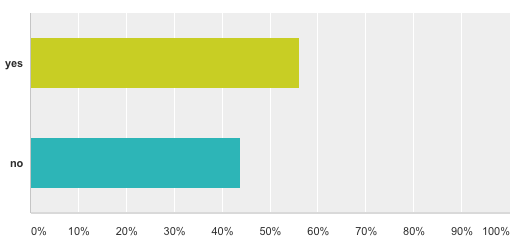
\includegraphics[width=100mm]{images/survey/analytics}
    \label{fig:label}
\end{figure}


The above survey gives an understanding on what users feel when using apps, also some insight into what they want to have more often. By asking a users these questions, it has given a meaningful reason to implement one of the key features to be implemented in the project. A feature that enables developers to keep the app updated quicker for users to feel like they are not forgotten, to give the app a new look and feel. But also a quick way to stop the user from deleting the app because it crashes. This will be further discussed in the design chapter.


% --------------------------------------------%
% Technologies researched
% --------------------------------------------%

\section{Technologies}

\subsection{Programming Languages}

\subsubsection{Objective-C}
Objective-C \cite{objectiveC} is an object-oriented programming language developed in early 1980s.  It was used to develop on NeXT OS which later became OSX and iOS.  Objective-C is a super set of the  C programming language meaning that it is possible to compile any C program with an Objective-C compiler. 

\subsubsection{Swift}
Swift \cite{swift} is Apple’s latest open-source programming language used mainly for developing on iOS, macOS, watchOS and tvOS applications.  Swift it an alternative to the Objective-C language, but is sometimes referred to Objective-C without the C. In contrast to Objective-C, it does not expose pointers to refer to object instances. Swift does retain Objective-C concepts including protocols, closures and enums. It was designed to make writing and maintaining programs easier for developers.

\subsubsection{Python}
Python \cite{python} is a high level programming language. It is designed to allow programmers to express concepts in fewer lines of codes than possible such as Java or C++. It is the perfect language to write programs on both a small and large scale. It supports object-oriented (OOP) and functional programming. Python was first created in the late 1980s by Guido van Rossum as a successor to the ABC language.

\subsection{Web Frameworks}

\subsubsection{Perfect (Server-side swift)}
Perfect \cite{perfect} is a web server and toolkit for developers using the swift programming language to build applications and other REST services. It can be deployed on macOS and Linux server.

\subsubsection{Kitura (Server-side swift)}
Kitura \cite{kitura} is a web server and web framework for Swift 3 developed by IBM. It is similar to Perfect, using core Swift technologies.

\subsubsection{Django}
Django \cite{django} is an open-source  high level Python web framework which follows the Model-View-Controller (MVC) pattern.  It consists of an object-relational mapper (ORM) that maps models (M)  defined as Python classes to a relational database, a system for processing  HTTP request to a web view (V).  It focuses on rapid development and the principle of  “don’t repeat yourself” and scalable. It was born in 2009 by few web developers and began to use Python to build applications. Django looks after authenticating the user when signing up, signing in and signing out. Python is used throughout the development even for setting files and creating models. Popular site such as Pinterest, Instagram and Bitbucket use Django for their web framework.

\subsubsection{Flask}
Flask \cite{flask} is a micro web framework written in Python and initially released in 2010. Applications such as Pinterest and LinkedIn use this framework. It is called micro framework as it does not require any dependencies to run, as well as that it does not have extra layers such as database but supports extensions that can be added to create extra features. Flask is popular among Python enthusiasts and was the most popular Python web framework on Github.

\subsubsection{Node.JS}
Node.JS \cite{node} is an open-source cross platform environment originally released in 2009. It is used to create a variety of tools and applications such as GoDaddy, Groupon and Paypal.  It is driven by events such as when a consumer purchases an item. Node.js has been optimized for web applications with many input/output operations, as well as real-time communication.

\subsection{Dependency Managers}

\subsubsection{CocoaPods}

CocoaPods \cite{pods} is the de facto standard of package management for iOS. It has the largest community and is officially supported by almost every open-sourced iOS library. It contains over twenty eight thousand libraries which are used in over 1.8 million apps.

\subsubsection{Carthage}

Carthage \cite{carthage} is intended to be the simplest way of add frameworks to apps. It was the first dependency manager for macOS and iOS, created by group of developers from Github. It was also the first dependency manager to work with Swift. It exclusively uses dynamic frameworks instead of static libraries, this is the only way to distribute Swift binaries that are supported by iOS 8 and up.

\subsection{Databases}

\subsubsection{MySQL}
MySQL \cite{sql} is an open-source relational database management system (RDBMS) initially released in 1995. Previously owned by a swedish company MySQL AB and now owned by Oracle Corporation. MySQL works on many system such as macOS, Windows, Linux, FreeBSD so making it a common choice and reviews are positive.

\subsubsection{MongoDB}
MongoDB \cite{mongoDB} is also a free and open-source database type program, but is a document-oriented. Classified as a not-only SQL (NoSQL) which uses JSON like documents to store objects. Features includes indexing, replication, load balancing and the list goes on. The main difference of MongoDB is that it is not a relational database. Objects that are related somewhat together are stored together in one file, improving retrieval of data.

\subsubsection{PostgreSQL}
PostgreSQL \cite{postgreSQL} is an object-relational database with additional object features. It differs itself support for highly required and integral object-oriented and relational database functionality, such as complete support for reliable transactions. It also free and open-sourced, yet very powerful with the capabilities of storing procedures.

\subsection{Web servers}

\subsubsection{Apache}
Apache \cite{apache} was created by Robert McCool in 1995 and has been furthered developed by Apache Software Foundation since 1999. The Apache web server has been the most popular server since 1996. Administrators choose this for its flexibility, power and widespread support. Apache creates processes and threads to handle additional connections. The admin can configure the server to control the maximum number of allowable processes, which is depending on the amount of physical memory. Each connects gets it own new thread which handles on user request.

\subsubsection{Nginx}
Ngnix \cite{nginx} was developed by Igor Sysoev in 2002, which answered to the problem that web-servers began handling ten thousands concurrent connection. It was initially released in 2004. Nginx has grown due to its light-weight resource utilization and its ability to scale. Nginx works different to Apache, in that it does not create new processes for each web request, instead the admin configures how many worker processes to create. The rule of thumb is that one work process for each CPU. Each worker can handle thousands of requests.

\subsection{Cloud Computer Services (IAAS)}

\subsubsection{Amazon Elastic Computer Cloud (EC2)}
%reword
EC2 " is a web service that provides secure, re-sizable compute capacity in the cloud. It is designed to make web-scale cloud computing easier for developers." \cite{ec2} Amazon EC2 is widely used by companies such as Netflix, AirBnB and Expedia. It can be used to launch as many or as few virtual servers as needed, that can be configured to suit your needs.

\subsubsection{DigitalOcean server}

DigitalOcean \cite{digital} is an American cloud infrastructure provider. It provides developers cloud services that help to deploy and scale applications that run simultaneously on multiple computers. As of December 2015, DigitalOcean was the second largest hosting company in the world in terms of web-facing computers. Within a few steps, you can have web-server up and running. The perfect choice for this project, that can set-up a Ubuntu 16.04 server in a matter of minutes. 

\newpage
\subsection{Evaluation}

% \usepackage[table,xcdraw]{xcolor}
% If you use beamer only pass "xcolor=table" option, i.e. \documentclass[xcolor=table]{beamer}
\begin{table}[!h]
\centering
\caption{Findings}
\label{my-label}
\begin{tabular}{|l|l|l|}
\hline
\cellcolor{green!20}Technology & \cellcolor{green!20}Version  & \cellcolor{green!20}Area \\ \hline
Swift      & 3.0.1      & Client Framework/Back-end Language \\ \hline
Linux      & 16.0.4 X64 & Server OS                          \\ \hline
MongoDB    & 3.2.11     & Cloud Storage                      \\ \hline
Flask      & 0.1.1      & Test Web Framework                 \\ \hline
CocoaPods  & N/A        & Dependency Manager                 \\ \hline
DigitalOcean    & N/A     & Cloud Service               \\ \hline
Nginx            & 1.10.3       & Web server               \\ \hline
Perfect            & 2.0      & Web Framework               \\ \hline
\end{tabular}
\end{table}

\subsubsection{Programming Language}

Chosen technologies as a result from the research for client side application is Swift for both the framework and dashboard app. I decided to go with Swift for client side programming for few different reasons but one that stood out was a blog from 9To5Mac website \cite{webserver}. At the beginning of 2016 Swift took over Objective-C making it the 14th most popular programming language. Protocol Oriented Programming (POP) is an interesting concept mainly used in Swift. It is starting to become commonly used instead of Object Oriented Programming (OOP) because objects are “things” that encapsulate complexity. So an object does it in a certain way, but protocols can provide objects with doing it different ways. With POP, the interface being what the user interacts with it the main and only concern.

\subsubsection{Dependency Managers}

A-Coding blog review goes into the pros and cons of both CocoaPods and Carthage \cite{acodingwebsite}. CocoaPods has a large community behind it, so problems can be easily help and resolved. There are a large number of available libraries and are listed on their website: https://cocoapods.org. It has a centralised file that manages all libraries required for the app along with version. But because it is centralized, if it goes down you will be affected.

Carthage is not centralised, each dependency is fetched from their original repositories. It can be very slow managing all dependencies, especially if the app requires a large number of them. Some find CocoaPods invasive as it modifies the Xcode project by building its own workspace. However Carthage does not, it is up to the developer to add the required libraries into their project.

Due to extensive help from the community, and the project is all about helping the developer with reducing the amount of development, the project will be using the CocoaPods dependency manager for the MBaaS framework.


\subsubsection{Web Framework}

The project is aiming to be open-source, so that developers can contribute towards it. So without needing to learn a different language like Python for Django, the choice is a web-server using Swift language. As swift is becoming more popular and has become open-source, it is reasonable conclusion that the near future will include more back-end servers written in swift.

Now the web framework choose it based on Swift programing language, the choice is between Perfect and Kitura. A bench-marks was conducted by Ryan Collins, a web developer. He posted a blog about the outcome \cite{benchmark} which clearly shows that not only is both Perfect and Kitura faster than Node.JS but that Perfect is the leader. The blog goes into detail of the test that was run, the server setup and the number of requests made.

\begin{figure}[!h]
    \caption{Benchmark}
    \centering
    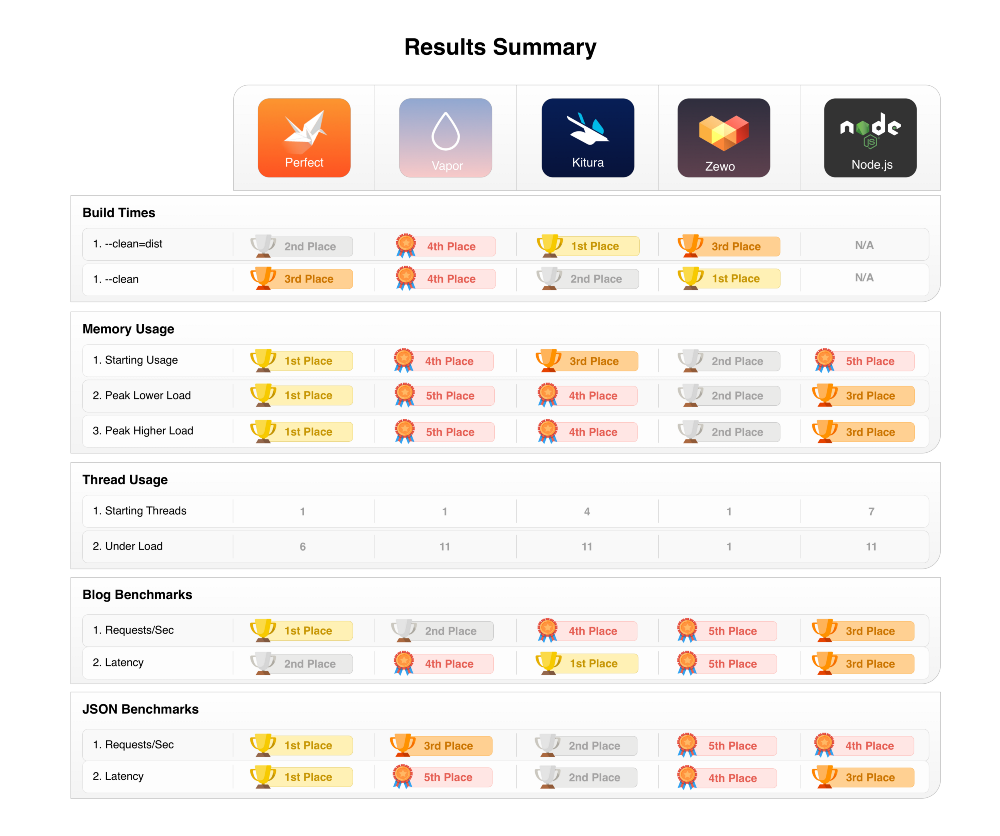
\includegraphics[width=75mm]{images/benchmarks}
    \label{fig:label}
\end{figure}

The result as stated in the blog, is that Swift is more capable of taking on the established server side frameworks. So regarding what Swift web framework to use, the decision is Perfect with over 10,000 stars on the Github repository. \cite{github1} 

\subsubsection{Database}
The database choice is MongoDB which is a NoSQL. It provides a dynamic way of storing data where object properties name and type are unknown until run time. This allows the system to be implemented with different types of data being sent and gives the developers less stress without having to worry about what models need to be created at design time. From the article “When to use MongoDB rather than MySQL” \cite{database} the reasons for choosing MongoDB is when:
\begin{itemize}
  \item Expect a high load amount of data
  \item Need to grow big 
  \item Do not have a database admin
\end{itemize}
The above 3 reasons are compelling enough to choose MongoDB because when designing a back-end as a service for applications of any type, then freedom and flexibility are key. Another valid reason is when you do not know the database structure and when providing a service to developers to give them tools to create any database structure is another strong reason to go with MongoDB. 

\subsubsection{Cloud Computer Services (IAAS)}
Digital Ocean

\subsection{Web servers}
Nginx has be decided for the project.

\subsection{Extra tools required}

\subsubsection{Xcode}

Xcode is an integrated development environment (IDE) containing a suite of software development tools developed by Apple for developing software for macOS, iOS and tvOS. First released in 2003, the latest version 8 is free download via Mac App Store. It supports source code for programming languages C, C++, Objective-C and Swift etc. 

\subsubsection{Swift Playgrounds}

Swift playground also know as just playground is an interactive work environment that allows you see the values in the sidebar for the written code. As and when you make changes to your code the sidebar reflects the changed result. It was introduced in Xcode 6 and enhanced in Xcode 7 that make learning Swift and experimenting much easier. Instead of having to create a app just to run and test some Swift code, a smaller playground can be made to view the outcome of each test piece. 

\subsubsection{APNs Auth key}

The Apple Push Notifications (APNs) involves generating an authentication key, that will sit on the server and will send notifications to one or more devices. Until recently, the generating of the authentication key consisted of painful steps. These include filling out a Certificate Signing Request in Keychain Access, then uploading it to your developer account. After which downloading a signed certificate, to which converting to .pem format. Also certificate would then expire, so the steps would need to be done again every year.

Now Apple has greatly improved this service, which involves the creation of one key of type .p8, which does not expire. The downloaded file, can then without converting be upload to the server to be used. Apple also gives three text keys that are used in authenticating the APNs and send the notifications. These include; APNs Auth key, Team ID and the App ID.

\subsubsection{Github}

Github \cite{github} is a web-based version control repository. It provides code sharing, publishing, deployment and much more. The developer can create as many private or public repositories as required. Github provides developers with tools to backup, version control and create branches to separate out builds.

\subsubsection{Perfect Assistant}
"This macOS companion application is a set of convenience tools designed to help Server Side Swift developers start, manage, compile, test, and prepare for deployment more easily. From those expanding into backend Swift development for the first time to seasoned senior engineers working on enterprise level projects, the Perfect Assistant will facilitate your work." \cite{perfectAssist} It is used to help include all the required packages required to build the project, and includes tools to deploy to amazon web-server and docker.


% --------------------------------------------%
% Similar Technologies researched
% --------------------------------------------%
% \newpage

\section{Similar Technologies}

\subsection{Overview}

\begin{table}[h]
\centering
\caption{Alternative Solutions}
\label{fig:overview}
\begin{tabular}{|l|l|l|l|l|}
\hline
\cellcolor{green!20}Service &\cellcolor{green!20}Parse &\cellcolor{green!20}Firebase &\cellcolor{green!20}BassBox &\cellcolor{green!20}Amazon \\ \hline
Notifications               & Yes                      & Yes                         & Yes                        & Yes\\ \hline
Database                    & Yes                      & Yes                         & Yes                        & Yes\\ \hline
Analytics                   & Yes                      & Yes                         & No                         & Yes\\ \hline
self hosted                 & Yes                      & No                          & Yes                        & No \\ \hline
Remote configuration        & No                       & Yes                         & No                         & No \\ \hline
Backup                      & No                       & No                          & No                         & No \\ \hline
User Sign-Up                & Yes                      & Yes                         & Yes                        & Yes\\ \hline
A/B Testing                 & No                       & Yes                         & No                         & Yes\\ \hline
\end{tabular}
\end{table}


\subsection{List}

\subsubsection{Parse}

\begin{figure}[!h]
    \caption{Parse}
    \centering
    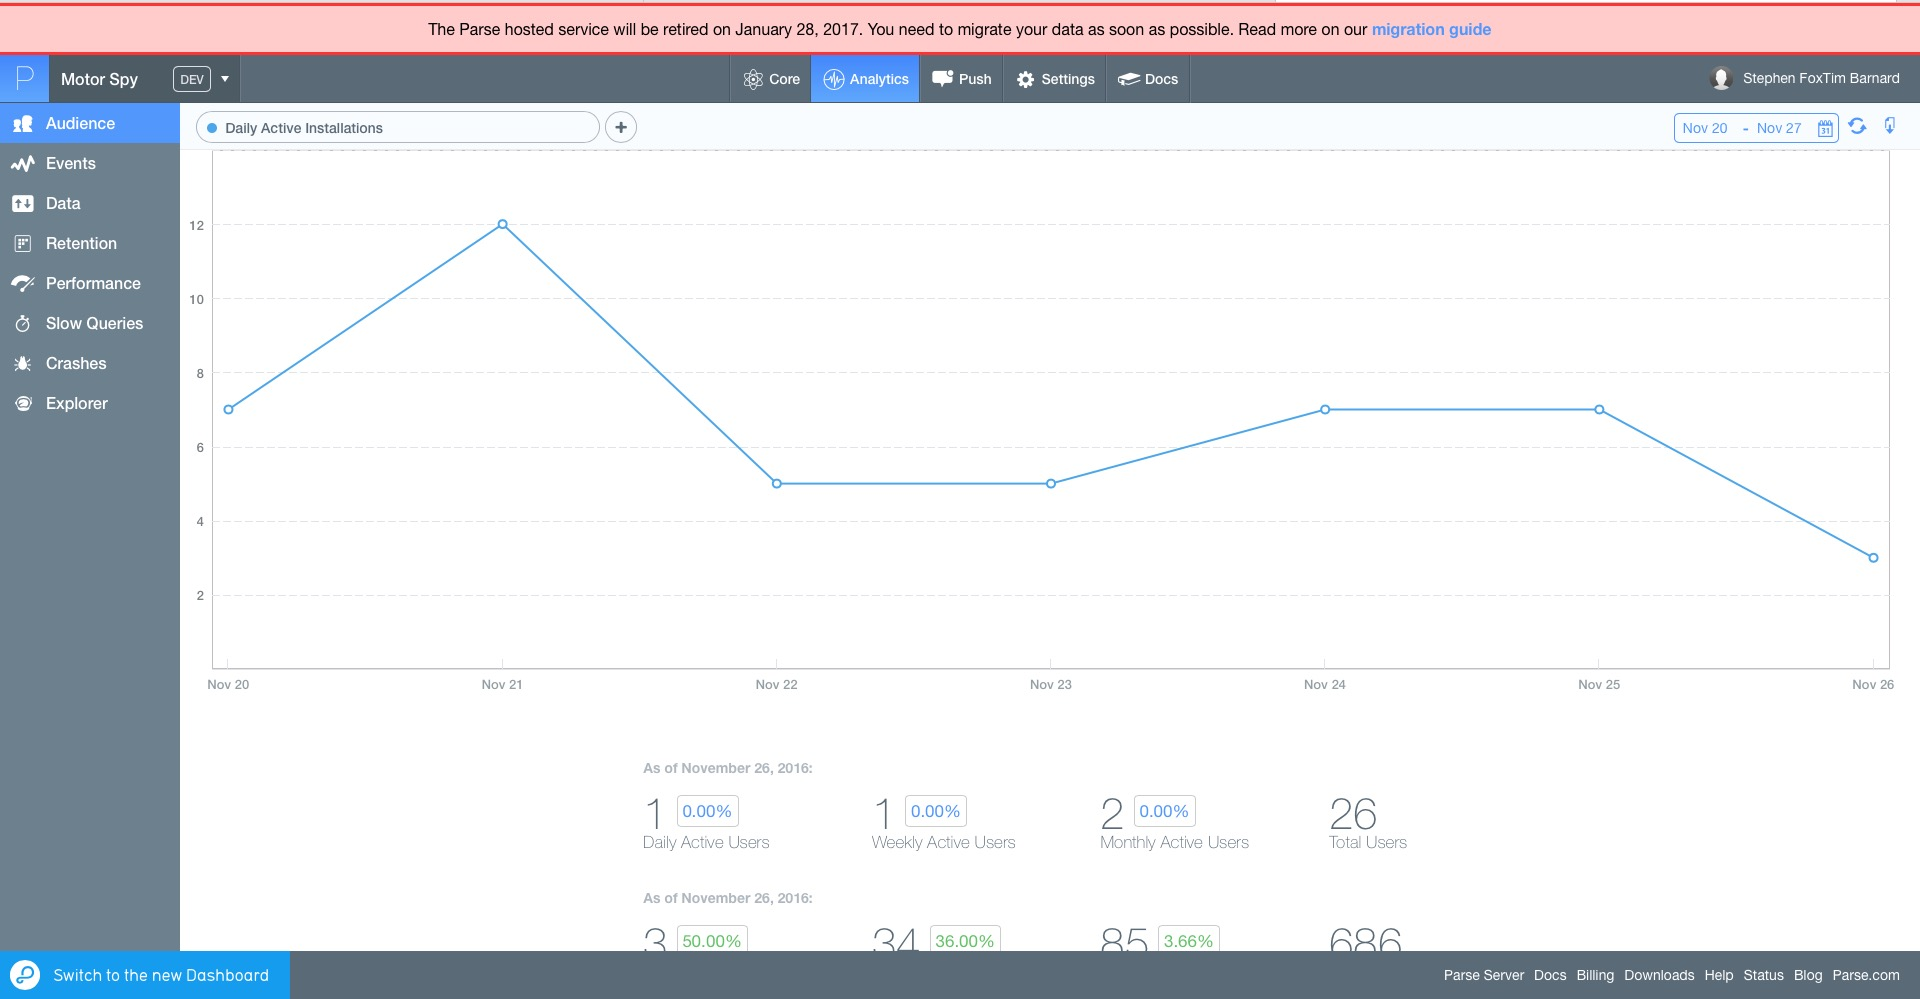
\includegraphics[width=100mm]{images/parse}
    \label{fig:parse}
\end{figure}

Parse \cite{parse} was founded in 2011 by Tikhon Bernstam, Ilya Sakhar, James Yu and Kevin Lacker former Google and Combinator employees. The project kick-started when it raised 5.5 billion dollars in funding in late 2011 and by 2012 over 20,000 mobile developers were using the service. Facebook in 2013 acquired the company for 85 million dollars and continued to grow. By 2014 500,000 apps were using the service, but sadly Facebook in 2016 announced that they are closing down the service in January 2017. They do provide tools and tutorials on how to migrate to your own hosted service. The service when operational was widely used by developers and Fig \ref{fig:parse} shows the main dashboard page. One of the developers mentioned in the interview that his company Tapadoo used to use Parse before they announced the closure of the service.

\subsubsection{Firebase}

\begin{figure}[!h]
    \caption{Firebase}
    \centering
    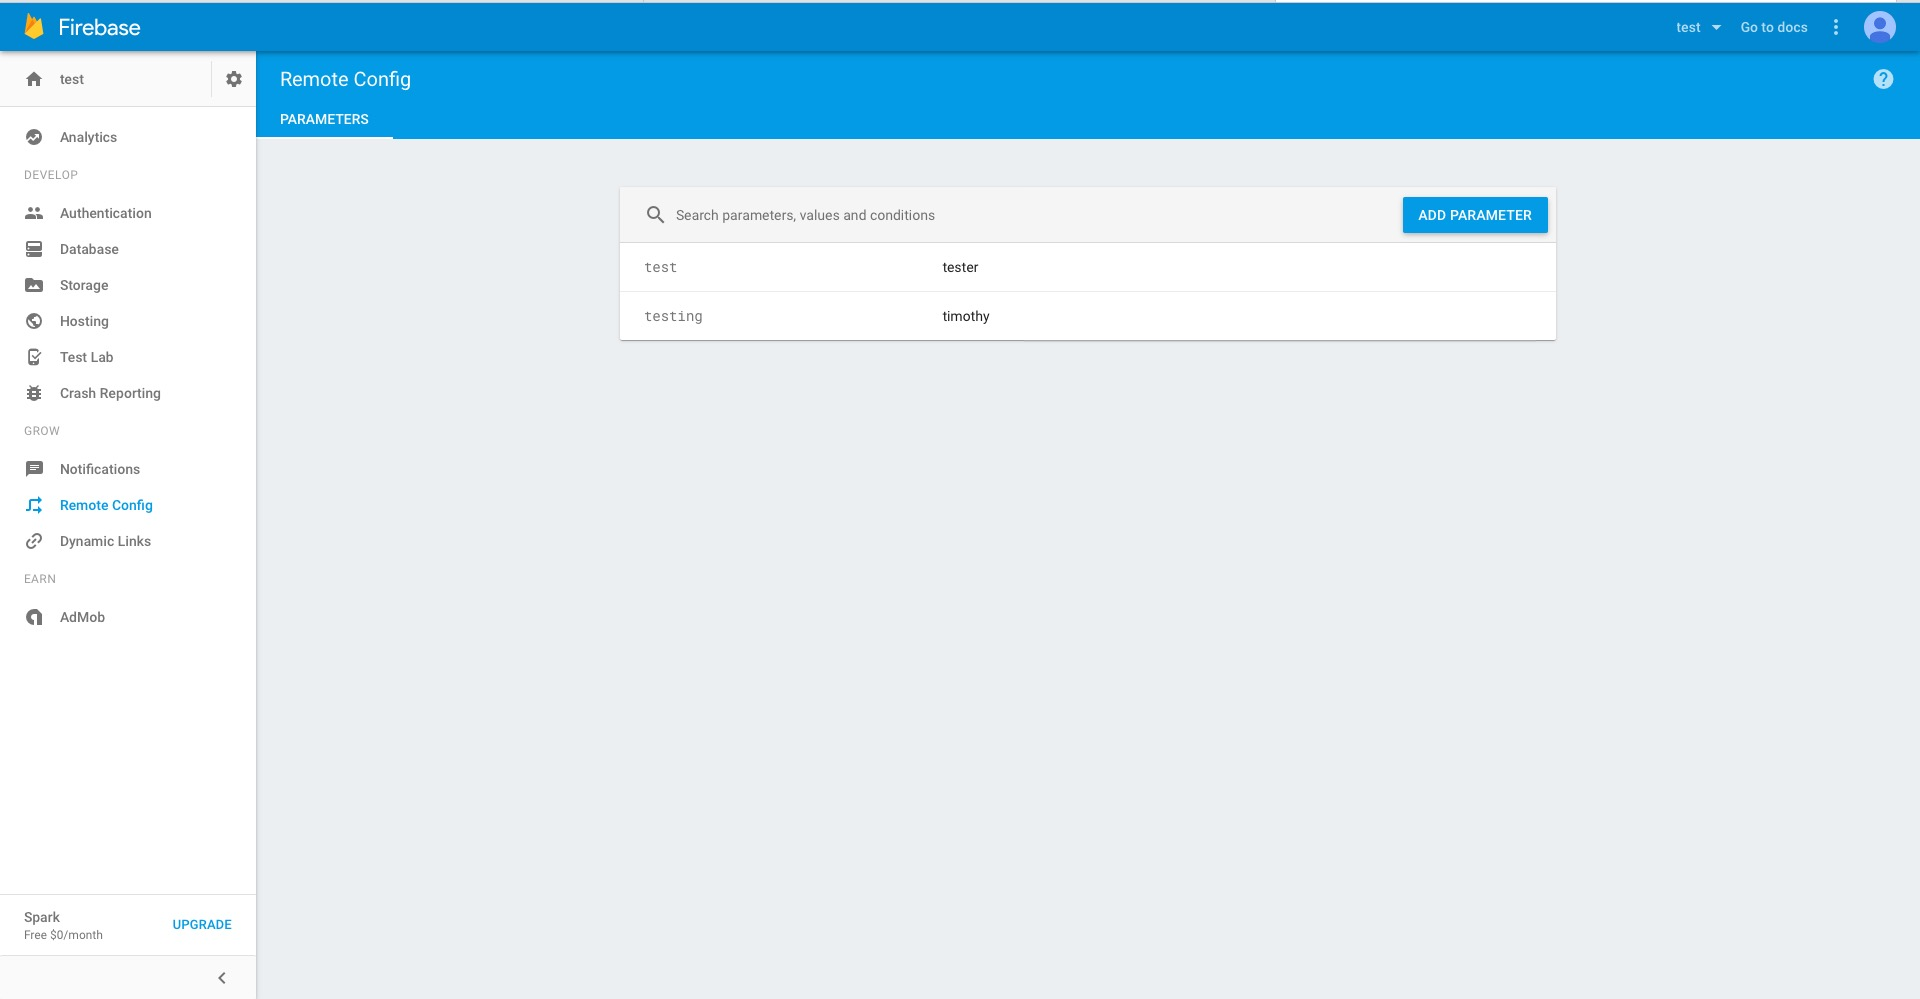
\includegraphics[width=100mm]{images/firebase}
    \label{fig:firebase}
\end{figure}

Firebase \cite{firebase}  evolved from Envolve, a start-up founded by Tamplin and Lee in 2011. They provided a service that enabled developers to integrate on-line chat into their web site but found after a while that the service was being used to pass application data that was not chat messages in real time. So the team decided to separate the chat system and real time architecture that powered it. This lead to the founding of Firebase, a separate company. 
It raised funding in 2013 and in 2014 Google acquired the company for an undisclosed amount. The company provides a list of services as shown in Table \ref{fig:overview} for free for limited amount of users and storage of 5GB, but as you increased the storage and users using your application then so does the price. If we way in more storage, real-time database space then the price per month is around 200 dollars \cite{firebase2}. The dashboard for managing your project is shown in Fig \ref{fig:firebase}, the current page is remote configuration service.

\subsubsection{BaasBox}

\begin{figure}[!h]
    \caption{BaasBox}
    \centering
    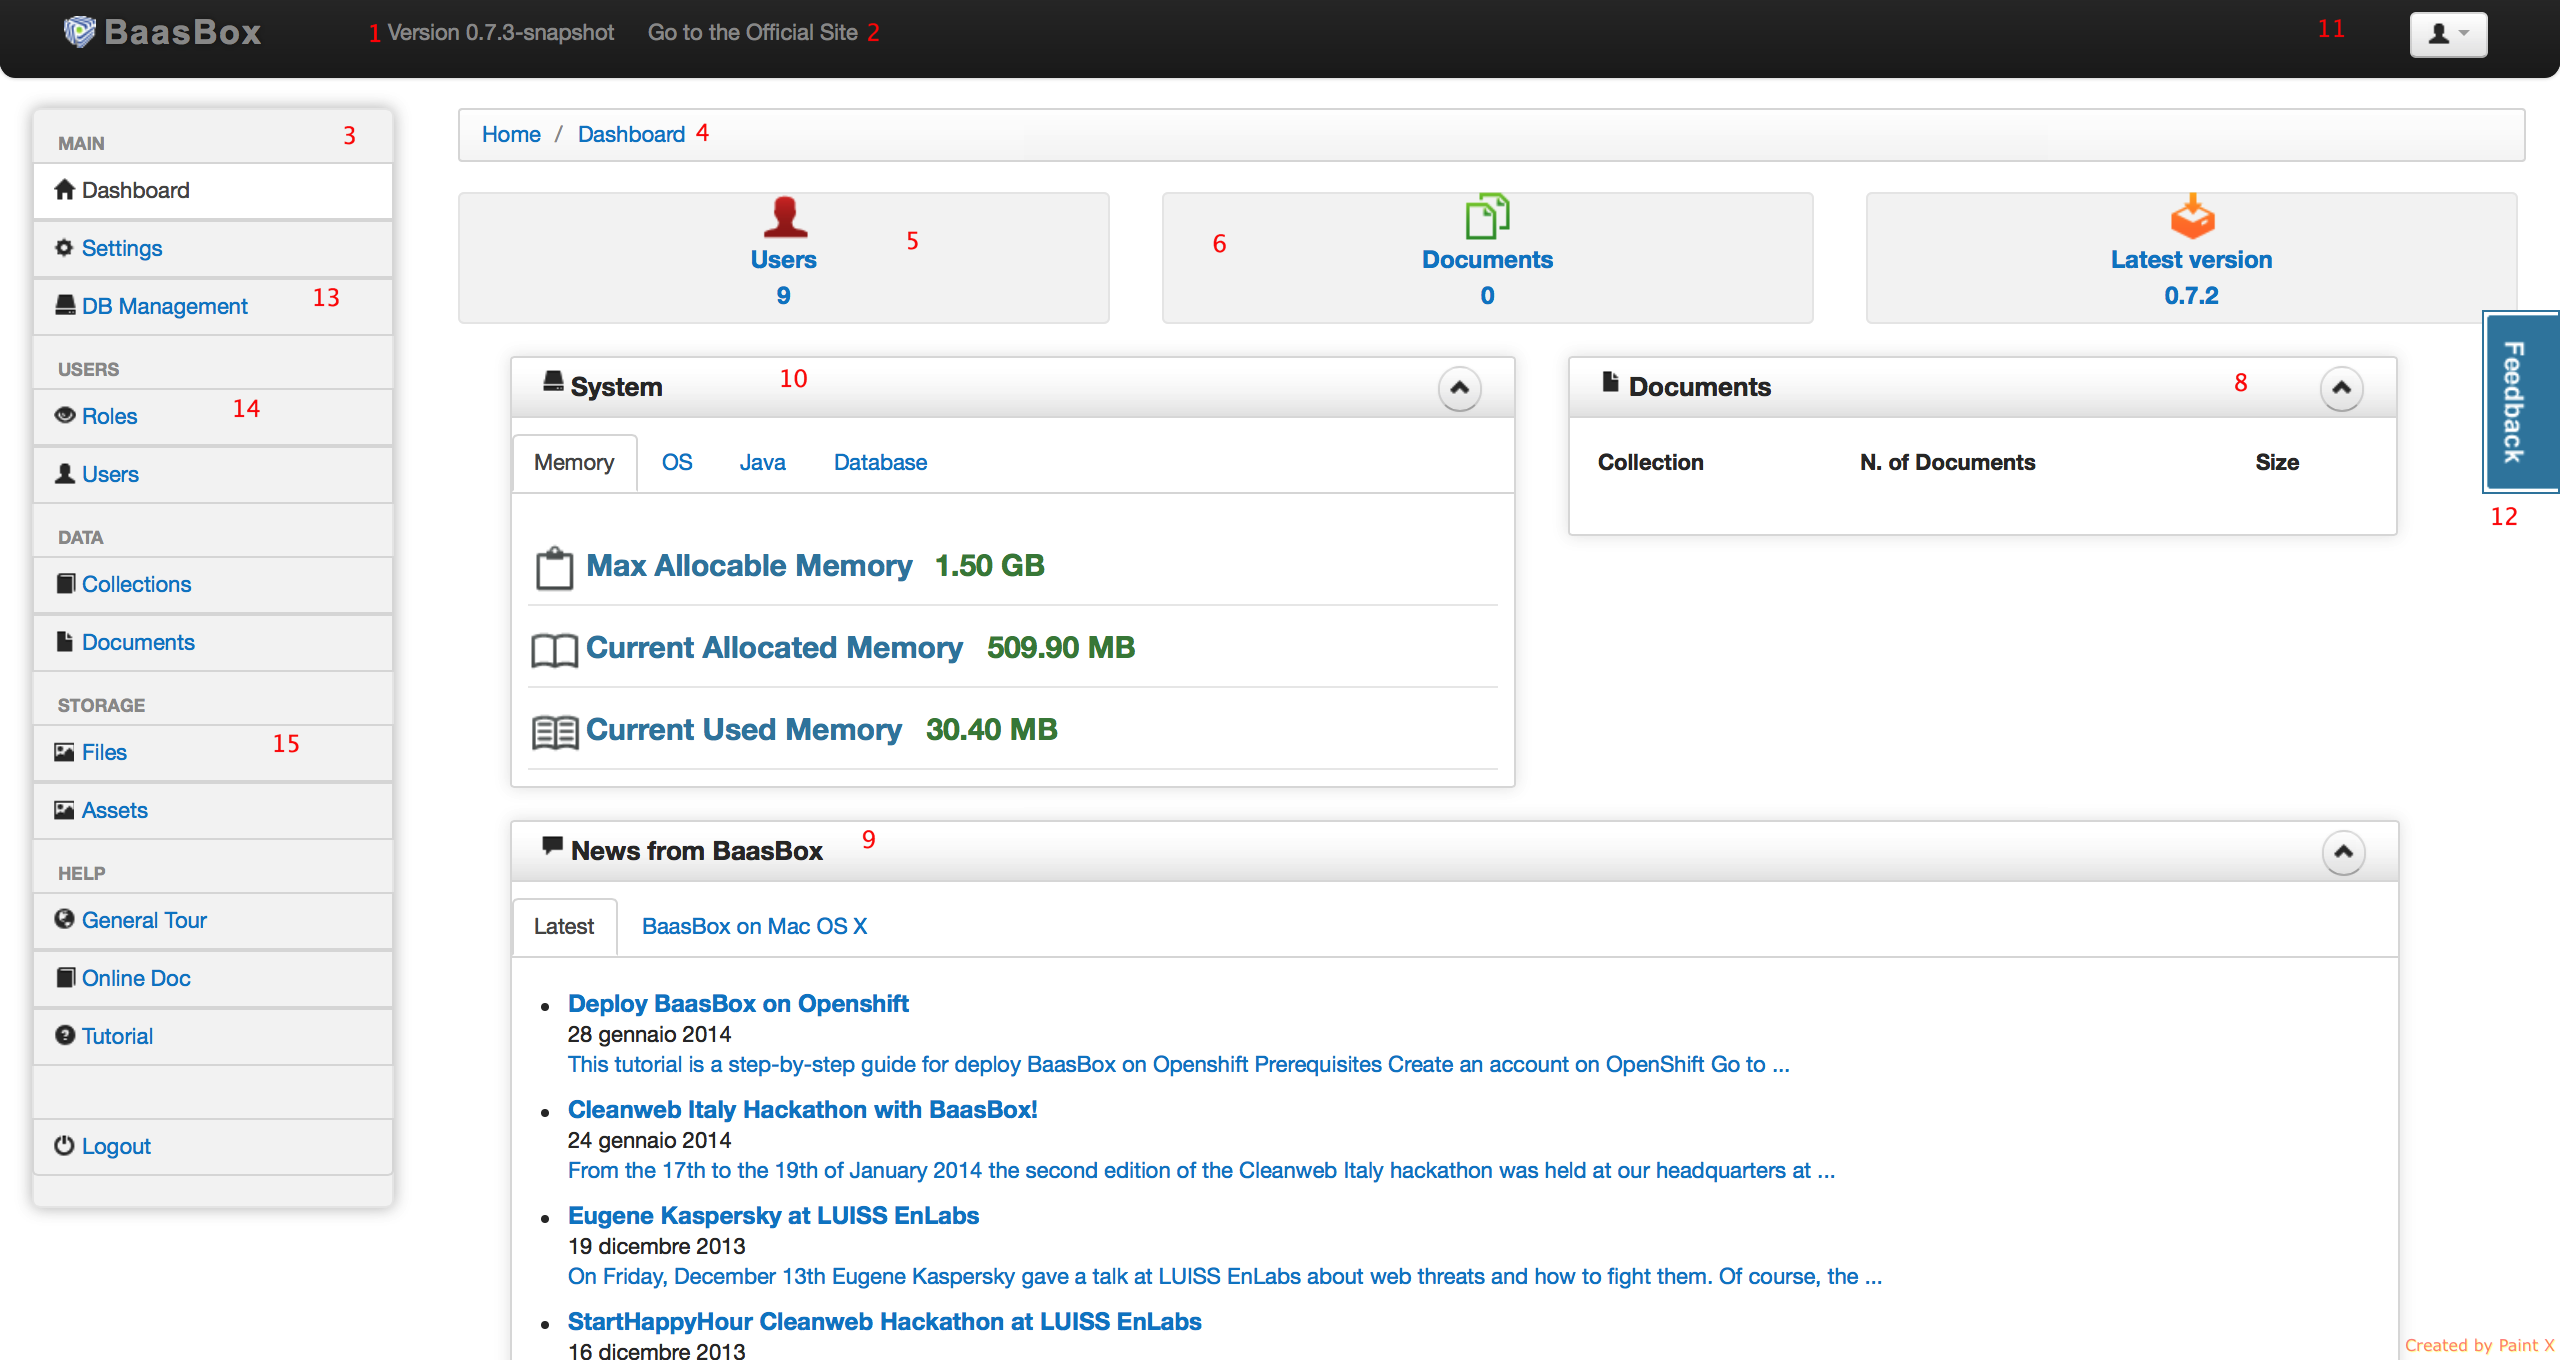
\includegraphics[width=100mm]{images/baasbox}
    \label{fig:baasbox}
\end{figure}

BaasBox \cite{baasBox} is an open sourced project founded in 2013, it is an application that acts a database and application server combined. It provides developers with an API as a back-end to store data for their mobile and web applications. It is the first back-end as a service to be open source and free to download. BaasBox also provides cloud services so instead of hosting the back-end on your own server. Fig \ref{fig:baasbox} shows the dashboard main page, on the left panel are a list of services they provide such as database.

\subsubsection{AWS}

\begin{figure}[!h]
    \caption{AWS}
    \centering
    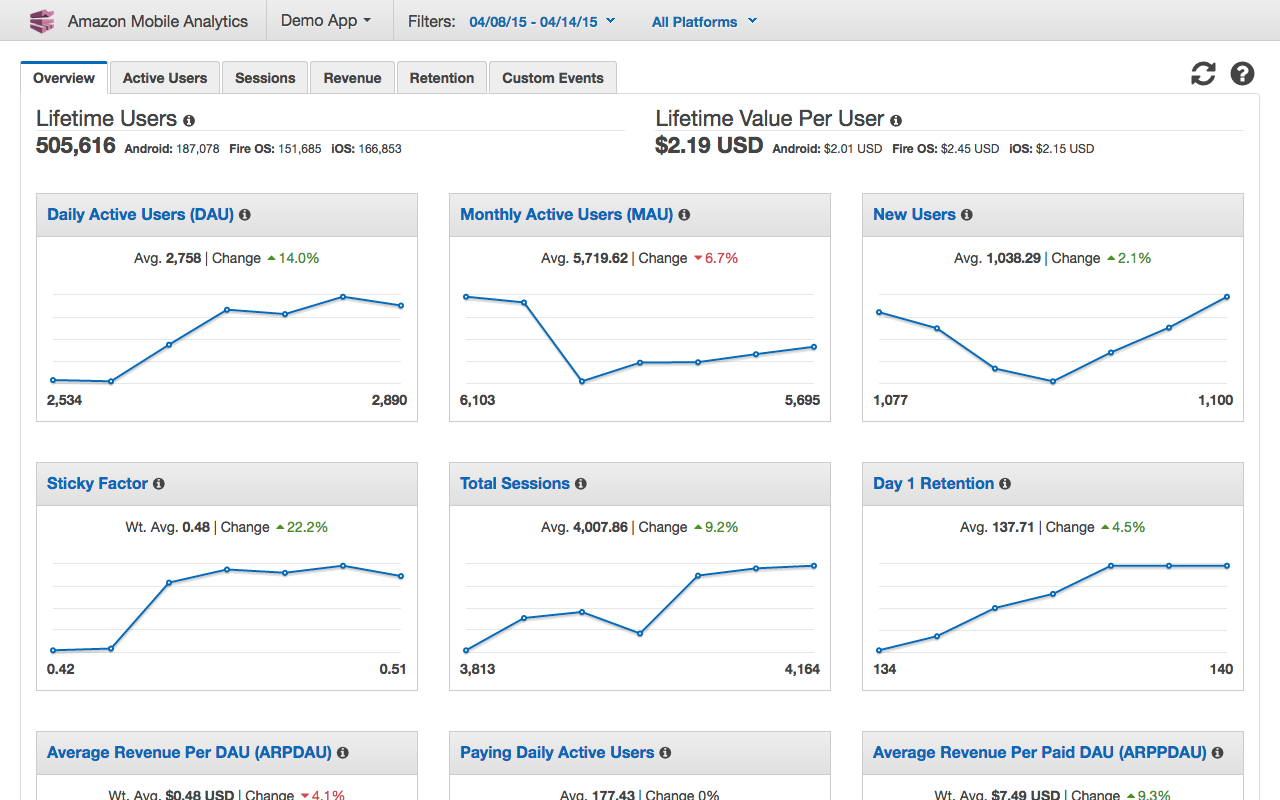
\includegraphics[width=100mm]{images/aws}
    \label{fig:aws}
\end{figure}

Amazon Web Services(AWS) \cite{aws} is a subsidiary of Amazon.com which offers a suite of cloud computing services launched in 2006.  By 2007 amazon claimed that more than 180,000 developers had signed up to use AWS Amazon Web Services. One of its services to AWS Mobile Services, a way to provide help to develop mobiles apps than can scale to hundreds of millions of users. Popular companies such as AirBnB and Netflix uses AWS mobile services to power their applications. Like other MBaaS providers, they do offer a limited 12 month free tier which includes 5GB of standard storage, 20,000 get requests and 2,000 put requests. Then outside of these limits the price does rise. The list of services they provide include analytics shown in Fig \ref{fig:aws}.


% --------------------------------------------%
% Requirements researched
% --------------------------------------------%
% \subsection{Requirements}

% After researching on similar technologies currently out their have lead me to the basic requirements. This include the following
% \begin{itemize}
%   \item Storage
%   \item Notifications 
%   \item Analytics
%   \item Sign up
% \end{itemize}

% Next came to part which is the reason why I wanted to do this project. A large challenge of a single developer without the money and resources for a design team, is struggling to think what end-users will like. This brought me to the next service requirement; A/B Testing. Also known as split testing is comparing two versions of a page to see which performs better.

\section{Human Computer Interaction}


% body of thesis comes here
\chapter{Design}

\section{Methodology}

\begin{figure}[!h]
    \caption{Tree-Shape}
    \centering
    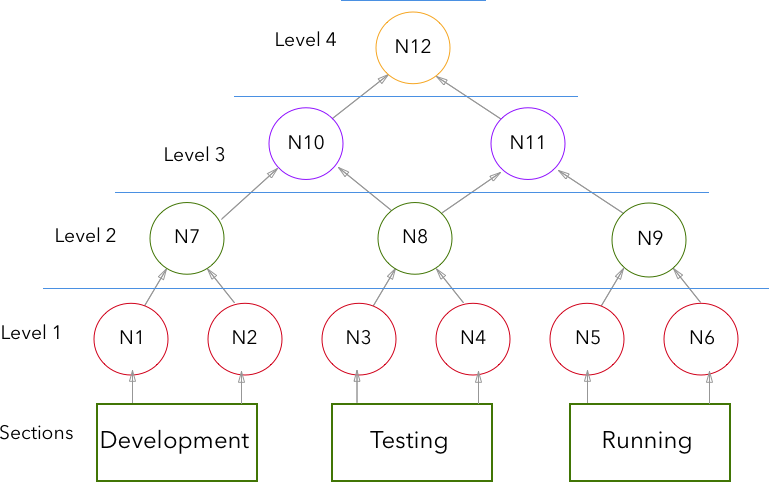
\includegraphics[width=100mm]{images/methodology}
    \label{fig:label}
\end{figure}

% \begin{figure}[!h]
%     \centering
%     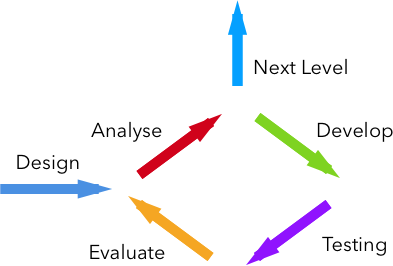
\includegraphics[width=50mm]{images/spiral_model}
%     \label{fig:label}
% \end{figure}

% \begin{figure}[!h]
%     \centering
%     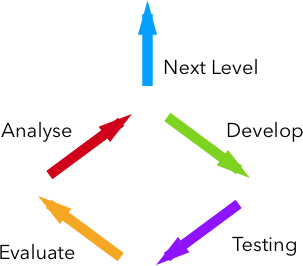
\includegraphics[width=50mm]{images/spiral_model_2}
%     \label{fig:label}
% \end{figure}

After doing research, I decided to implement my own methodology called "Tree-Shaped". The idea behind this methodology is to en-corporate the functionality into different sections, and prove each functionality at a lower, early stage. This benefits by setting out the goal into sections and filling in what functional requirements are need to reach the goal. The proving of functionality part is to able to fix any potential compatibilities at an earlier stage or remove if necessary.

The methodology has three parts

\begin{enumerate}
  \item Sections
  
    The sections stage is first step in using the "tree shaped" methodology. This part is where we set out what we are trying to achieve. Then incorporate each functionality into their respective sections.
    
  \item Functionality   
    
     After we define our sections including their respective functionalities, tests are to be written out for each functionality. This are to show that they still output the correct result, being what they are supposed to do.
    
  \item Levels
  
    Levels stage is where we are proving/testing the functionalists. As we move up the tree into each node, the functionalists are combined together. Thus solving compatibilities issues at an earlier stage of the project development.
\end{enumerate}

\subsection{Advantages}

This methodology is based on the test-driven development (TDD) process that relies on the repetition of very short development cycles. At each level, the nodes which holds the application are tested. These tests are from the functionality part, when combining the previous nodes, we want to make sure they still output the correct result.

\subsection{Disadvantages}

The methodology although sounds good from a theoretical point of view, but in a real world it has its drawbacks. Each node (circle in each level) requires making new test application, combing the previous two node applications and potential re-factoring. This takes time where some projects do not have, but we reduce the number of bugs found but re-factoring at each level. To overcome this, the methodology allows to skip one level to reduce testing times.

\section{Functional Requirements}

Functional requirement defines a function of a system or its component. After talking to out-sourced developers and researching current systems out there, the following table \ref{tb:functional} defines the list of functional requirement. They are grouped into sections and what the aim of the project will deliver.

\begin{table}[h]
\centering
\caption{Functional Requirements}
\label{tb:functional}
\begin{tabular}{|l|l|l|l|l|}
\hline
\cellcolor{green!20}ID & \cellcolor{green!20}Section  & \cellcolor{green!20}Name  & \cellcolor{green!20}Description        & \cellcolor{green!20}Priority \\ \hline
1                      & Development                  & Database storage          & Create, Read, Update, Delete objects   & High   \\ \hline
2                      & Development                  & Push notifications        & Send push notifications to devices     & Medium \\ \hline
3                      & Production                   & Analytics                 & Measure users in app activities        & High   \\ \hline
4                      & Production                   & Backup                    & Backup database to remote site         & Low    \\ \hline
5                      & Production                   & Self hosted               & Host the MBaaS on developers server    & High   \\ \hline
6                      & Production                   & Remote Configuration      & In app live updates                    & High   \\ \hline
7                      & Production                   & A/B Testing               & Testing different variations           & High   \\ \hline
8                      & Development                  & Live Database             & Update objects without user refreshing & Low    \\ \hline
9                      & Development                  & Dashboard                & Interface for developers manage apps   & High   \\ \hline
10                     & Testing                      & Exception catching      & Interface for developers manage apps   & High   \\ \hline
\end{tabular}
\end{table}

\subsection{Development}

\subsubsection{Database}

The API and framework will provide a service to send and retrieve objects to the  database. These tools will not only be able to post and get objects but also to set out filters.

\subsubsection{Self hosted}
Allow the developer to host their own system to have full control on when up and running, and not having to worry if the provider is going to shut down the system. By giving the developer a way to host their own back-end then this will keep the cost down of not having to paying for third party services.

\subsubsection{Backup}
This feature gives the developer a piece of mind that the applications data is constantly backup to local or remote location.

\subsubsection{Sprint board}
Challenge faced when creating an application, is trying to keep a list of features or changes to be made for a version. Also knowing history of features already implemented. Their are already different sprint board applications out there, but I wanted a way to en-corporate it all in one single dashboard app, that can be used with teams.

\subsection{Testing}

\subsubsection{Crashes}

\subsection{Production}

\subsubsection{A/B Testing}
A/B testing also known as split testing is comparing two versions of a page to see which performs better. Currently this popular with web pages but my plan is to bring this to mobile applications. All mobile applications no matter what services they provide all have one goal; a reason to exist. A/B testing allows you to make more out of your existing traffic. This is achieved by sending our to variants ( A and B ) to similar visitors at the same time and use analytics to provide us what version wins. Included in my research, I did a survey to see how end-users respond to different applications. How they look?, Are they concerned on the aesthetics of the app?. At stated end-users do choose whether or not they will continue to use an app. So by using A/B testing service we can quickly find out what they do and do not like. So how can we implement this service in mobile apps? This leads on to my next service.

\subsubsection{Remote Configuration}
Remote configuration is a service that lets you change the behaviour and appearance of the app without requiring the users to download an app update. When using this service, you create the default appearance such as how a button looks, whats the title etc. Then later on we can update this values via the dashboard to configure these. So how does the app know when to get the new version? Included in each request done within the app is the configuration object at the top. This object will tell you, what version is available to download. So why use remote configuration? 
\begin{itemize}
  \item Quickly roll out changes to your app
  \item Customise your app depending on the version they are running
  \item Use this along with A/B testing to find improvements
\end{itemize}

\subsubsection{Notifications}
Allowing the developer to reach their users and perform tasks in the background. These allows the developers to bring the attention of the users to their app if for example a message comes in. A powerful tool to keep the app in real time and the user connected to the app. Ability to add notification certificates relating to each applications and to send individual or bulk notifications.

\subsubsection{Analytics}
Analytics to give the developer real time information on how their app is doing, how users are using their app. Custom tool to configure what data they want to analyse for example, if the applications is based on vehicles then it can be configured to show list of top vehicle type, make or model. Each configuration will have a graph on the main screen. Analytics will also be used for AB Testing service explained later.

\subsection{Non Functional Requirements}

\subsection{Security}
Security is a big part to any cloud based applications. Users personal information being sent up to cloud, where potential hacks could expose these. Not along has able enforcing developers to user HTTPS request, to secure data transmission, I have also taken into account some security measures. 

\subsubsection{Keys}
The systems supports two keys authentication, there is one key that allows requests to access the web server services. The next key allows data back and fourth to the database.

\subsubsection{Database}
Instead of all applications the developer owns being contained in one database, each application created gets their own database. These are only allowed access once the key gets authenticated.

\section{Deliverables}

\subsection{Dashboard}

\subsubsection{Storage}

Figure \ref{fig:storage_use_case} illustrates storage/database in use cases. In the storage view in the dashboard, the developer will be able to choose a database which is specific to each application. After which be able to view and select the collections within, and see the content records. Another feature is the ability to import collection from a JSON or CSV file into the database.

This use case is limited by design, the typical create, read, update and delete (CRUD) operations known with database development will not be available. When designing systems that include both backend and frontend, the most important one of two is the frontend. This is what the end users will see, so this system will focus on designing the structure of each collection in the application, in development stage. Typically the dashboard will allow the developer to perform CRUD operations, and then they will have to mimic that structure for the frontend app, thereby creating a potential bug. A bug can occur if someone is able to change the collection name, or collection property name, thus creating an inconsistency between frontend and backend. Removing the capabilities from one side being backend will hopefully remove this potential issue. 

\begin{figure}[!h]
    \caption{Storage Use Case Diagram}
    \centering
    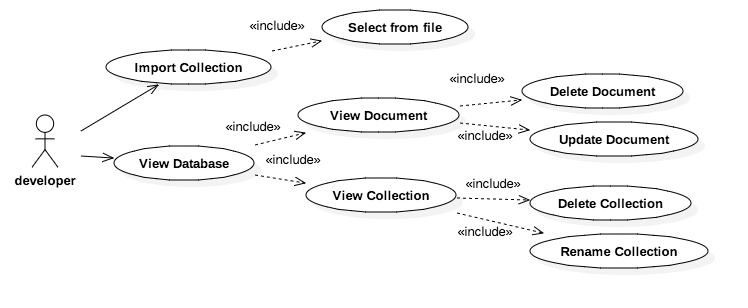
\includegraphics[width=100mm]{images/use_cases/storage_use_case}
    \label{fig:storage_use_case}
\end{figure}

\subsection{SDK}

\subsubsection{Storage}

\begin{table}[!h]
\centering
\caption{SDK Storage Design}
\label{tb:storage_design}
\begin{tabular}{|l|l|}
\hline
\rowcolor{green!20}
Functionality                  & Result                \\ \hline
protocol for each object       & parsing objects to and from JSON \\ \hline
convert objects to JSON        & JSON string \\ \hline
parse collection into object   & collection of objects \\ \hline
send object to server          & unique record id      \\ \hline
filter when retrieving objects & filtered objects      \\ \hline
\end{tabular}
\end{table}

The table \ref{tb:storage_design} shows the functionality requirements and result for the storage part in the library. The first functionality being the protocol, which will give all structures that same functionality. The development chapter later will go into detail how the protocol works.

\section{Design Principles}
Human Computer Interaction (HCI) principles plays a major role when designing an interface. These principles help keep applications of the same nature alike. An example is a mail app, the icon for mailbox or sending messages can be used to convey without having to read a manual of what a button does. As this system will be using a mac application, apples macOS interface guidelines will be closely followed.

Apples Human Interface Guidelines \cite{guidelines} discussed the following design principles:

\begin{enumerate}
  \item Mental Model 
  
  - "..is the concept of an object or experience that people carry in their heads". It is the model of what users believes about the system, so the mental model of past experience on similar systems will be carried when looking to use this system. This will involve looking at current systems available and design the interface somewhat similar.
  
  \item Direct Manipulation
  
  - "..is an example of an implied action that helps users feel that they are controlling the objects represented by the computer". When designing a view that the user can control, the objects such as deleting a record, should only become invisible once the user has taken the action.
  
  \item User Control 
  
  - "..principle of user control presumes that the user, not the computer, should initiate and control actions." The interface should give the user the control depending on the type of user. So an professional user will want more control compared to novice user.
  
  \item Consistency
  
  - "..allows the user to transfer their knowledge and skills from one app to another". So by designing the system will the same general layout of other apps will help the user not feel lost.
  
\end{enumerate}
\chapter{Architecture}

\section{Overview}

\begin{figure}[h]
    \caption{Overview}
    \centering
    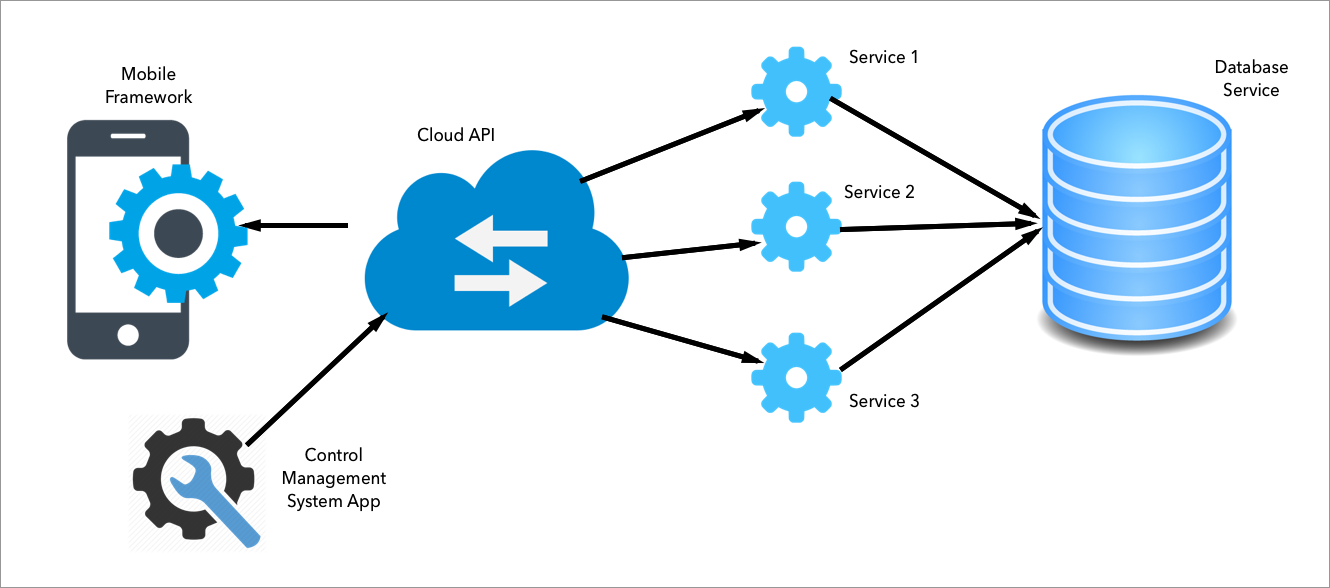
\includegraphics[width=100mm]{images/overview}
    \label{fig:label}
\end{figure}

Figure \ref{fig:label} illustrates the overview architecture of systems, and the four main parts required. The first being the web-server that provides a cloud based service, that takes requests and performs the necessary task. The next part which follows on from the web-server is the database, to store data persistently. This also provides a cloud based database so that data can be accessed from anywhere. The third part being the mobile framework which creates the communication to the web-server through an API which will be discussed later in this chapter. The framework separates the complexity of the web-server system, and provides easy to use tools to communicate. The last main part is the control management system app, which provides an interface to configure the web-server and display the current set-up.

\section{Web Architecture}

\begin{figure}[!h]
    \caption{Four-tier Architecture \cite{ted} }
    \centering
    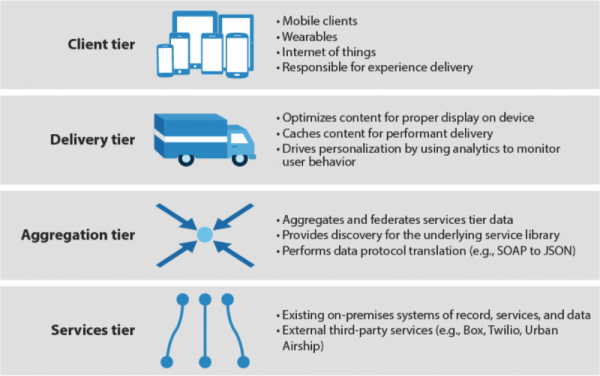
\includegraphics[width=100mm]{images/four-tier}
    \label{fig:four-tier}
\end{figure}

The Four-Tier Engagement Platform is the chosen web architecture for my project shown in Fig \ref{fig:four-tier}. The client tier allows the development of an application without having to worry about the backend services. Delivery tier gives the consumer the best possible mobile experience by caching content locally on the device app so if service is lost then they can still use the app. The aggregation tier connects the apps to the correct services with bi-directional, real-time data from the back-end. Finally the service tier gives the other tiers the data they require. It is used to also integrate current services already being used by the company such as MySQL or MongoDB. 

\section{Back-end as a Service}

\begin{figure}[!h]
    \caption{Client Server Diagram}
    \centering
    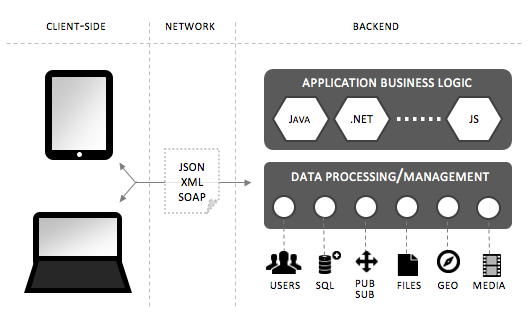
\includegraphics[width=100mm]{images/client-server-diagram}
    \label{fig:client-server}
\end{figure}

Applications today are put into the category of "client-server apps" where the applications consist of client-side(frontend) and the server-side(backend). The client-side is what the user see, what type of device it is, being computer or mobile apps. The client-side is responsibility for show the data to user in some sort of interface, along with taking their requests and passing it to the server. 
The backend consists of two primary components: application business logic and data processing/management. The data processing/management operates on various resources being users, persistent data, files etc. The business logic manages triggering notifications based on changes in the data, prevent unauthorised access.  Figure \ref{fig:client-server} illustrates this.

\subsection{API}

In order for the applications to communicate with the back-end, there needs to be a common based protocol that defines how data flows. Thus combining the protocol with the data structure definitions created an Application Programming Interface (API). The typical format used in most applications is called  Representational State Transfer REST which is an architectural style and approach to communications used in web services development. REST provides a list of verbs such as GET, POST, DELETE in which request can be made using HTTP. The diagram \ref{fig:api} below illustrates this: 

\begin{figure}[!h]
    \caption{API}
    \centering
    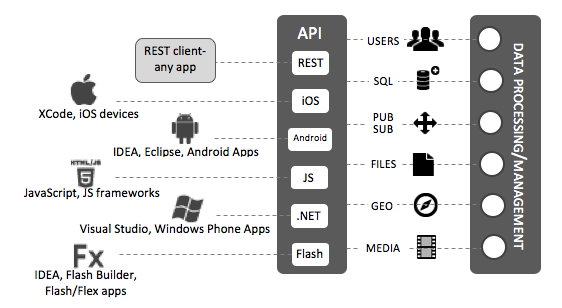
\includegraphics[width=100mm]{images/baas-apis}
    \label{fig:api}
\end{figure}



\chapter{Development}

\label{ch:conclusions}

\section{Introduction}

As explained in the design chapter, this project includes three deliverables. So the development will include; a Mac app dashboard, Perfect web-server and CocoaPods framework. Using the "tree-shaped" methodology the web-server was split up into their separate sections which include development, testing, and run. Then each service was design, developed and testing before moving up the tree. The development then broken up into phases, this way the project can be kept on track on what has been completed and whats left to do.

\begin{enumerate}
  \item Services Development
  \item Integrate into Live App
  \item Dashboard Development
  \item CocoaPod Framework 
\end{enumerate}

As this project methodology is based on Test Driven Development (TDD) approach, the services was developed first and tested before adding to the project. Then once these services have cleared, they were integrated into the DIT-Timetable app explained later, this was to ensure how the new services were developed would pass Apples prepublish tests. Once this was accomplished, the dashboard was developed next to view the services in an interface. Then lastly the services were developed into a SDK to be used in any mobile application.

\section{Project Management}

Good software project management is essential in developing and delivery of software projects. Software development is often difficult to estimate the time required to complete the project, especially when using new technologies. Project milestones can be used to monitor the development progress of the project at certain key points. Above includes the list of the key points within the project. Each point had its own time frame; this kind of project can lead to expanding to including more services and tools, so sticking to the list will help be on schedule.

This project differs from commercial project, in that the project manager, designer, developer and tester were all the same person. And with any project, testing plays a major role in software development and can easily be left out. So self-discipline was required as there was no "boss" to answer to. 

\section{Services Development}

Each service had it's own Perfect server application along with Playground app. This made is easy to decide whether or not it was possible to implement each service into the project. For some of the services, the same Perfect web-server was used and able to be adapted to accommodate the requests needed. 

\paragraph{Setup} Before any development was started, some services was required to be setup. Perfect web-server developers provides an "assistant" to help with the setup and include and required packages needed to develop the API. The list of packages for the project include the following:

\begin{enumerate}
  \item https://github.com/PerfectlySoft/Perfect-Turnstile-MongoDB.git
  
  -Used to provide functionality to interact with MongoDB database, and provide authentication when requests come to the server.
  \item https://github.com/PerfectlySoft/Perfect-RequestLogger.git
  
  -Provides the web-server with a logging system.
  \item https://github.com/hkellaway/Gloss.git
  \item https://github.com/PerfectlySoft/Perfect-Notifications.git
  
  -Aid with the push notifications.
  \item https://github.com/PerfectlySoft/Perfect-SMTP.git
  
  -To be able to send Mails
  \item https://github.com/PerfectlySoft/Perfect-Zip.git
  
  -To zip backups folders, when sending to remote location.
\end{enumerate}

After the Perfect web-server was setup, the mongoDB was required to installed locally. This was done by running the following commands in list \ref{lst:mongodb}

\lstinputlisting[label={lst:mongodb}, language=Bash, caption=MongoDB setup]{development/code/mongo.m}


\lstinputlisting[label={lst:playground},language=Swift, caption=Playgrounds setup]{development/code/playground.m}

To be able to run asynchronous code in the playgrounds, the following lines of code in list \ref{lst:playground} is required to be added to the top of the file. This will to make asynchronous code and get results.

\subsubsection{Database storage}

The database storage section is split up into two parts of the development. 

\begin{enumerate}
  \item Object-relational mapping (ORM)
  \item Storage - how to send the objects to store persistently
\end{enumerate}

\paragraph{ORM}

The database storage required an object role model (ORM) which is a powerful method for designing and querying database models at the conceptual level, where the application is described in terms easily understood by non-technical database developers. It is a technique for converting data between incompatible type systems in object-oriented programming languages. The ORM was developed using Playground tool, where the creation of objects and parsing into JSON objects. The functionality of the ORM is to create a new object, parse it and send to the server, and be able to bring all objects back from the server.

This was developed using protocols and protocol extension. Protocols as Apple states "defines a blueprint of methods, properties, and other requirements that suit a particular task or piece of functionality." and extensions are "new functionality to an existing class, .., protocol type.". \cite{protocol} A protocol called TBJSONSerializable was developed as seen in listing \ref{lst:protocol_ext}

\lstinputlisting[label={lst:protocol_ext},language=Swift, caption=Protocol]{development/code/protocol_ext.m}

The first protocol TBJSONRepresentable simply states that this variable TBJSONRepresentation has to be used in any class or protocol conforming to that protocol. Inside the TBJSONSerializable protocol, we have two methods that any class or structure used throughout any mobile application will have to these two methods. The TBJSON to a type alias that is a dictionary, which holds the JSON objects which will be used when parsing. Next the protocol extension was developed, where the objects will be parsed into a dictionary type form that then can easily be parsed in JSON. In listing \ref{lst:TBJSONSerializable} illustrates how the objects are parsed.

\lstinputlisting[label={lst:TBJSONSerializable},language=Swift, caption=TBJSONSerializable]{development/code/TBJSONSerializable.m}

In listing \ref{lst:TBJSONSerializable}, the TBJSONRepresentation variable contains a switch case to loop through the mirrored; which is a representation of the sub-structure, each class property such as String, Int or Dictionary, and depending on the type be parsed into AnyObject and assigned to the dictionary with the key being the name of the variable.

The design also stated that in reprieving objects, functionality is to be in placed to parse back to objects. Using protocol extension to type alias of dictionary and method chaining, a list of functions was implemented to parse each value back to the desired type. The method chaining speeds the development time for the developer, without needing to find the correct type first. An example of this is in listing \ref{lst:tryConvert} which takes the parameter of the key, and tries to parse the value in two ways. First if the value if of type integer, it will return that value, but if it is of type String, it will convert string to integer and return the new value.

\lstinputlisting[label={lst:tryConvert},language=Swift, caption=Dictionary]{development/code/tryConvert.m}

\paragraph{Storage}

As part of the project architecture with regarding to storage, any structure should have the functionality to send to the server, and retrieve without the need to create another function to setup and communication over HTTP. As described in the design chapter, all structures conforming to the protocol will be able to send and retrieve the object/s between the server and the application. JSON is used in the transfer of data, a format in which both server and client can understand. JSON objects are simply just dictionaries where each value has an object of some type. The following table \ref{tb:object} illustrates the library commands to send and retrieve objects between the cloud storage. The T in the return column means that this function return type is of a certain type. In the following examples will be returning type TBJSONSerializable which is our protocol.

\begin{table}[!h]
\centering
\caption{My caption}
\label{tb:object}
\begin{tabular}{|c|l|c|l|}
\hline
\rowcolor{green!20}
\multicolumn{1}{|l|}{Library Method} & Description & \multicolumn{1}{l|}{Parameters}                                                       & Result            \\ \hline
getFilteredInBackground                                      & \begin{tabular}[c]{@{}l@{}}Retrieves the filtered\\ object\end{tabular} & \begin{tabular}[c]{@{}c@{}}query: {[}String:AnyObject{]}, \\ type:T.Type, \\ appKey: String = ""\end{tabular} & T Object          \\ \hline
getInBackground                                              & Retrieves the object                                                    & \begin{tabular}[c]{@{}c@{}}objectID: String, type:T.Type, \\ appKey: String = ""\end{tabular}                 & T Object          \\ \hline
removeInBackground                                           & Removes the object                                                      & objectID: String, appKey: String = ""                                                                         & Successful/ Error \\ \hline
sendInBackground                                             & \begin{tabular}[c]{@{}l@{}}Update or send the \\ object\end{tabular}    & \multicolumn{1}{l|}{objectID: String, appKey: String = ""}                                                    & Successful/ Error \\ \hline
\end{tabular}
\end{table}

The next table \ref{tb:objects} illustrates returning back array of objects.


\begin{table}[!h]
\centering
\caption{My caption}
\label{tb:objects}
\begin{tabular}{|c|l|c|l|}
\hline
\rowcolor{green!20}
\multicolumn{1}{|l|}{Library Method} & Description & \multicolumn{1}{l|}{Parameters}                                                       & Result            \\ \hline
getFilteredInBackground                                      & \begin{tabular}[c]{@{}l@{}}Retrieves the filtered\\ object\end{tabular} & \begin{tabular}[c]{@{}c@{}}query: {[}String:AnyObject{]}, \\ type:T.Type, \\ appKey: String = ""\end{tabular} & T Objects \\ \hline
getAllInBackground                                           & Retrieves the object                                                    & \begin{tabular}[c]{@{}c@{}}objectID: String, type:T.Type, \\ appKey: String = ""\end{tabular}                 & T Objects \\ \hline
\end{tabular}
\end{table}

\begin{figure}[!h]
    \caption{Storage Sequence Standard}
    \centering
    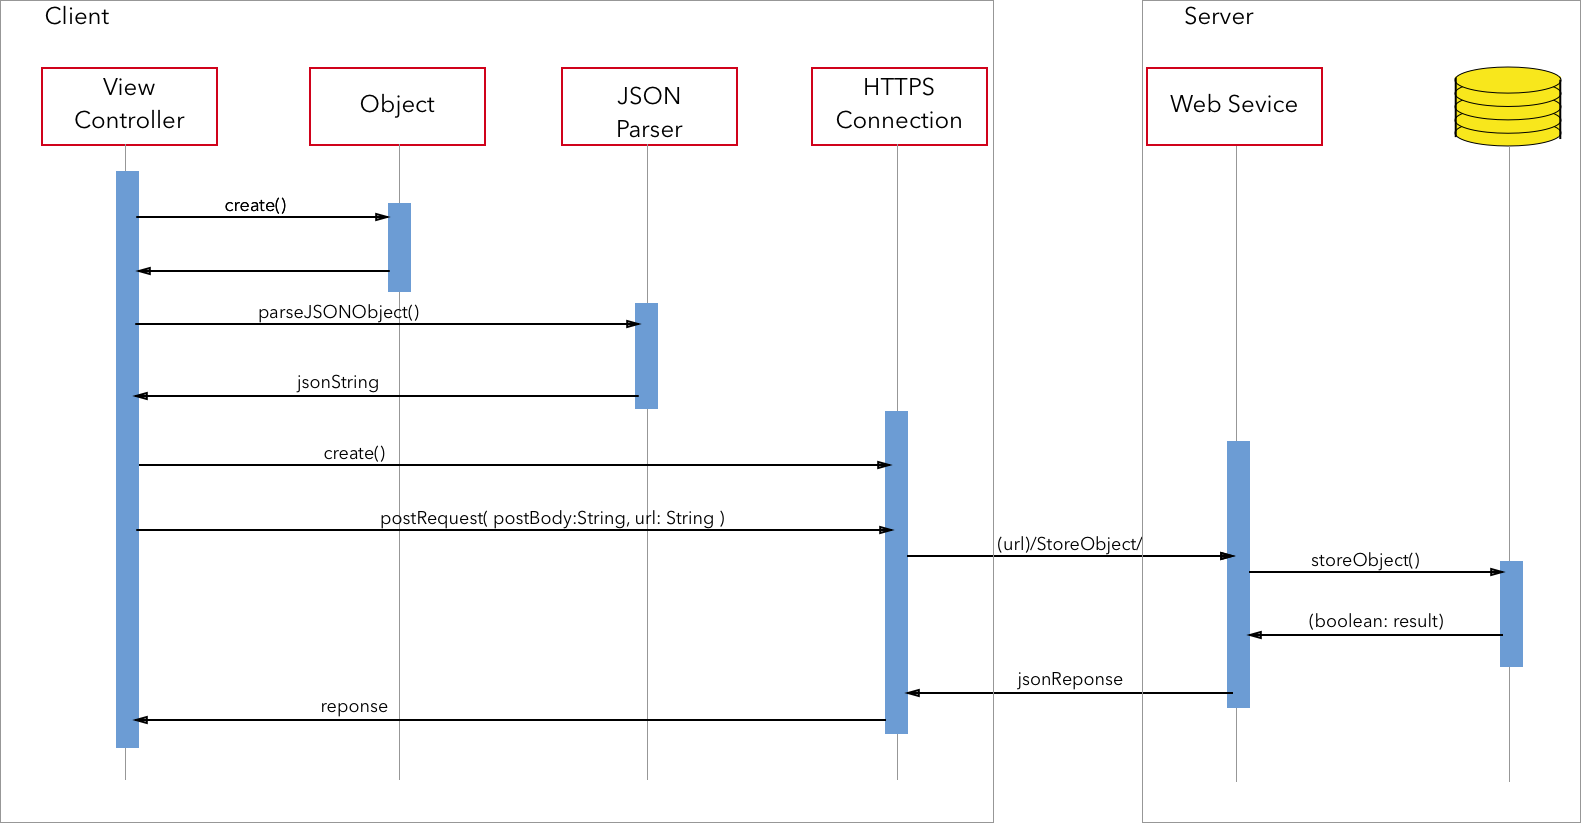
\includegraphics[width=100mm]{images/services/storage_sequence_current}
    \label{fig:storage_old}
\end{figure}


\begin{figure}[!h]
    \caption{Storage Sequence New}
    \centering
    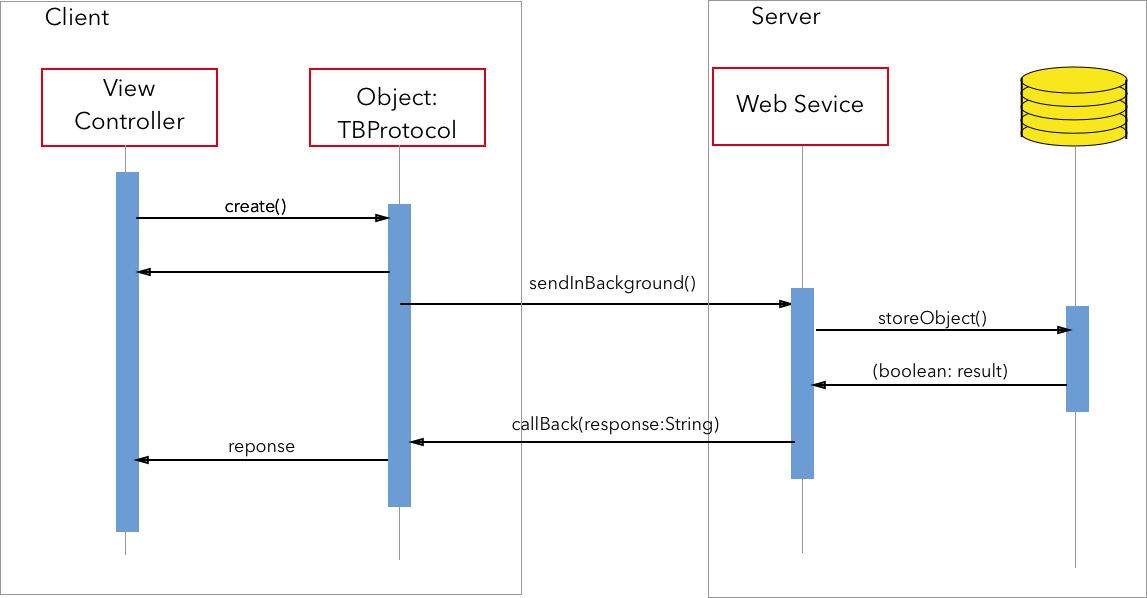
\includegraphics[width=100mm]{images/services/storage_sequence}
    \label{fig:storage_new}
\end{figure}

The two figures \ref{fig:storage_old} and \ref{fig:storage_new} show the difference to developing the standard way, with the developing having to create a JSON parser and then set-up a HTTPS connection to send it to the server in Fig \ref{fig:storage_old} . The new way in Fig \ref{fig:storage_new} using the project's storage protocol involves the developer only having to create the object, then using the objects functionality to send it to the server.

\subsubsection{Apple Push Notifications (APNs)}

\paragraph{Server}

Push notifications requires a number of steps to be implemented. First the .p8 key was downloaded, then the Perfect server test project required accessing that file to send notifications. Using the DIT-Timetable app to receive the push notifications.  

\begin{figure}[!h]
    \caption{APNs \cite{apns}}
    \centering
    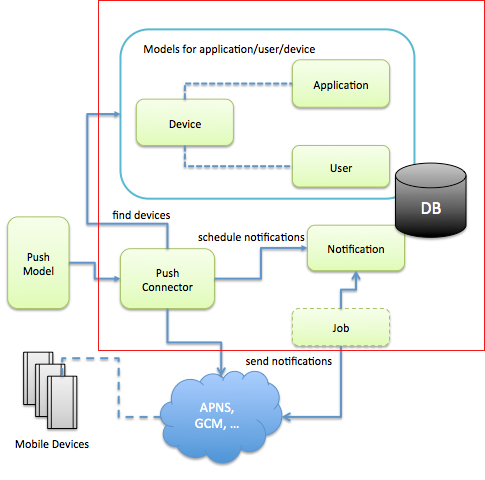
\includegraphics[width=75mm]{images/APNs}
    \label{fig:apns}
\end{figure}

In fig \ref{fig:apns} represents the stages in which to send push notifications. Inside the red box is the server layer, where the .p8 file is located, the push model is where the messages come from. The notifications goes through Apple's sandbox APNs, then on to the mobile devices.

\paragraph{Client}

APNs tool was implemented in the library, for which the developer can use the notification object to send request to the server, which in turn sends the notifications. The notifications object requires a list of values to be set for the notifications to work.

\begin{itemize}
  \item Universally Unique Identifiers
  - the targets device unique id to which apple will the notification
  \item Message
  - message which source wants to send to the target
  \item Badge Number
  - each notification can be assigned a number, which display on the app icon
  \item Title
  - the title of the notification, usually the app name
\end{itemize}

The following table \ref{table:mob_apns} demonstrates notification library to send notifications.

\begin{table}[!h]
\centering
\caption{APNS Library}
\label{table:mob_apns}
\begin{tabular}{|c|c|c|c|}
\hline
\rowcolor{green!20}
Library Method                    & Description                        & Parameters    & Result              \\ 
\hline
TBNotification.sendNotification();        & \makecell{Sends notifications\\ object to server} &  None & Successful/ Error   \\ 
\hline
\end{tabular}%
\end{table}

Fig \ref{table:apns} shows how to use the API requests outside of the library.

\begin{table}[!h]
\centering
\caption{Analytics API Requests}
\label{table:apns}
\begin{tabular}{|l|l|l|l|}
\hline
\rowcolor{green!20}
API Call                        & HTTP Method & Description                    & Parameters   \\ \hline
/\{appKey\}/notification & POST        & send notification object       & JSON Object  \\ \hline
/\{appKey\}/storage/TBNotification & GET         & Retrieves all notification objects & JSON Objects \\ \hline
\end{tabular}
\end{table}


\subsubsection{Analytics}

The first part for the analytic developed was the creation of the Perfect web-server which excepted POST requests. A playground application was developed with the lines of code in list \ref{lst:playground} to aid with HTTP requests. This class made gathers some information before sending the request, this include, time-stamp, build version, OS version, device make and model. For the purposes of testing this service, the data was hard-coded in separate function, that in turn would be reading from plist file. Some of methods and the parameters are included in the following table \ref{table:mob_analytics} shows how to use the library to send analytics. The server stores the analytic objects in the database corresponding to the application, this is done using the appKey which is sent up in the API request.

\begin{table}[!h]
\centering
\caption{Analytics Library}
\label{table:mob_analytics}
\begin{tabular}{|c|c|c|c|}
\hline
\rowcolor{green!20}
Library Method                    & Description                        & Parameters    & Result              \\ 
\hline
TBAnalytics.sendOpenApp();        & \makecell{Sends up object\\ with open app type} &   \makecell{view: UIView , \\ method: String? = \#function \\ , file: String? = \#file } & Successful/ Error   \\ 
\hline
TBAnayltics.send();               & \makecell{Send up object \\ with type as option} &  \makecell{ app: UIResponder, \\ type: SendType \\ , method: String? = \#function ,  \\ file: String? = \#file } & Successful/ Error   \\ 
\hline
 \makecell{ TBAnayltics \\.getAllInBackground(); } & \makecell{Retrieves all \\ TBAnayltic objects }   & NONE        & Array of TBAnayltics \\ 
\hline
\end{tabular}%
\end{table}

Fig \ref{table:analytics} shows how to use the API requests outside of the library.

\begin{table}[!h]
\centering
\caption{Analytics API Requests}
\label{table:analytics}
\begin{tabular}{|l|l|l|l|}
\hline
\rowcolor{green!20}
API Call                        & HTTP Method & Description                    & Parameters   \\ \hline
/\{appKey\}/storage/TBAnalytics & POST        & Uploads analytics object       & JSON Object  \\ \hline
/\{appKey\}/storage/TBAnalytics & GET         & Retrieves all analytic objects & JSON Objects \\ \hline
\end{tabular}
\end{table}


\subsubsection{Remote Configuration}

The remote configuration service development is broken up into four sections.

\begin{itemize}
  \item JSON files 
  - where the configuration objects will reside on the phone
  \item JSON file manager
  - how we will retrieve the values
  \item Objects configuration
  - how each interface object can be configured
  \item Remote change
  - will be discussed in the dashboard development
\end{itemize}

This section will discuss the first three, the remote change will be explained in dashboard development section.

\paragraph{JSON files}

The first part was the development of the JSON file layout. The design chapter already discussed the design of the remote configuration, where each class object will contain the objects relating to that class, and subsequently the objects properties will be in the object. To help with this, the storage protocol TBJSONSerializable was used to be able to parse the objects into JSON string. In listing \ref{fig:rc-cd} illustrates the class diagram for the complete remote configuration structure.

\begin{figure}[!h]
    \caption{Remote Config Class Diagram}
    \centering
    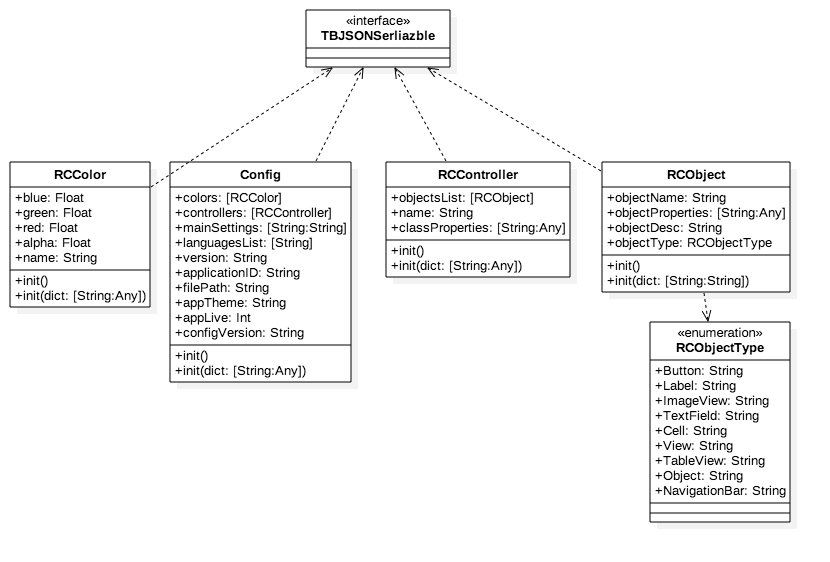
\includegraphics[width=150mm]{images/classdiagrams/config}
    \label{fig:rc-cd}
\end{figure}

In figure \ref{fig:rc-cd}, the remote configuration structure consists of 5 classes. The very first class of the structure is the Config class. This is where all the other class objects will be located. The config class holds a number of properties, the first being the colors value, where all colours used in the application will be stored. The RCColour object contains the RCG values along with alpha and the name of each colour. This name will be used in the properties of each object for example background colour. Next is controllers of type RCController, these are the main classes or commonly known as ViewControllers in the mobile app. 

Moving on to the RCController class, the properties include the name for that class which is the same name in app, the class properties so for example, if that class is of type UIViewController, that class will contain backgroundColor property etc. The last property is objectList of type RCObject. This is where all objects such as labels, text fields, tables etc will be stored. The RCObject class contains the name of the object, along with its own properties, these are what are provided by the framework when developing an app. The object type property is a type of enumeration which will contain what base class name is for example UILabel. The reason for this will be explain later in the dashboard development section.

Back to the Config class, the main setting are key value pairs that hold main data such as URLs, these are stored at this level to speed up retrieval. The language list are as the name states, contains the list of translation languages that the end user can change. This will be explained later in the language service section.

% \lstinputlisting[label={lst:config},language=Swift, caption=Configuration Structure]{development/code/config.m}

% In listing \ref{lst:config} lines 3 - 6 inclusive, holds the configuration objects for the applications. The colours objects is where all colours used in the app will be, this was placed here to speed up retrieval of each colour. The controllers objects is an array of view classes used within the app, then subsequently not shown are the objects within each class, and the properties relating to each object. The mainSettings variable on the same line of colours was placed here to speed up the retrieval of any import key values in the app such as URL. Last the languages list holds the list of languages available to the application. The languages part is based on the same as configuration files.

% Lines 8 - 13 are to distinguishes this configuration file with another, so when an update of configuration is done, then the application call tell if it has the latest or needs to download. This is to stop re-downloading the same file over and over again. The following listing \ref{table:json_manager} shows the library methods which to use the remote configuration files.

\paragraph{JSON file manager}

\begin{table}[!h]
\centering
\caption{JSON file manager}
\label{table:json_manager}
\begin{tabular}{|c|c|c|c|}
\hline
\rowcolor{green!20}
Library Method                    & Description                        & Parameters    & Result              \\ 
\hline
RCConfigManager.getColor();        & \makecell{retrieval of\\ colour} &   \makecell{ name: String, defaultColor: UIColor } & UIColor   \\ 
\hline
 \makecell{RCConfigManager\\.getTranslation(); }  & \makecell{retrieval of\\ translation value} &  \makecell{  name: String, defaultName: String  } & String  \\ 
\hline
\makecell{ RCConfigManager \\.getMainSetting(); } & \makecell{retrieves main\\ setting value  }   & \makecell{  name: String, defaultName: String } & String \\ 
\makecell{ RCConfigManager \\.getObjectProperties(); } & \makecell{retrieves object\\ properties  }   & \makecell{  className: String, objectName: String } & [String:AnyObject] \\ 
\hline
\makecell{ RCConfigManager \\.getConfigVersion(); } & \makecell{gets latest version\\ of config file  }   & None & call back method \\ 
\hline
\makecell{ RCConfigManager \\.getConfigThemeVersion(); } & \makecell{gets latest version\\ of config theme file  }   & None & call back method \\ 
\hline
\end{tabular}
\end{table}


\paragraph{Objects configuration}

Object configurations involves how to get the object properties and update the user interface (UI) object. In the design chapter, it was discussed that a protocol along with protocol extension will be used on each UI object. A separate protocol for each UI object will be developed. To do this, a protocol is first define, then an extension on that protocol to add the implementation. A snippet example of UILabel UI Object is in the following listing \ref{lst:protocol}

The extension LabelLoad is restricted for classes with type UILabel, and the developer has two methods it can use to implement. Inside the setup first, the object properties is retrieved from the JSON files, and then set to the corresponding property value.

\lstinputlisting[label={lst:protocol},language=Swift, caption=UILabel Protocol]{development/code/protocol.m}

\subsubsection{A/B Testing}

A/B Testing utilizes two other services, remote configuration and Analytics. Using the JSON files, it can tell us what version of configuration is being used, so when an analytic object is sent up, then we include the version. The server however needs some development to handle A/B Testing. The dashboard explained later is used to set what applications, version of time the testing will be done. When a request comes into the web-server for configuration file, a check on the A/B Testing list is done to check whether that app version exists as seen in figure \ref{fig:abtesting-cd}. 

\begin{figure}[!h]
    \caption{A/B Testing Class Diagram}
    \centering
    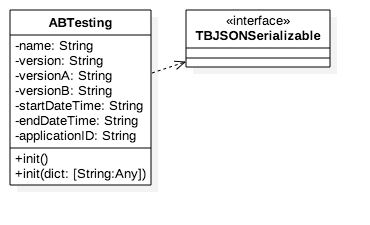
\includegraphics[width=100mm]{images/classdiagrams/ABTesting}
    \label{fig:abtesting-cd}
\end{figure}

The class diagram comprises of the ABTesting table along with the protocol TBJSONSerializable mentioned earlier. The table properties include the name of the testing, the application id and version for which that testing is part of. The versionA and versionB are the two different configuration files, and the dates for which the testing is in place.

To develop this service on the server, a singleton class "RemoteConfig" is used. When the server starts up, the singleton class is initialized with a current request number of zero. With each request, the count increases, and using this value can depend on what version of the configuration file that users gets.

% \subsubsection{Live Database}

\subsubsection{Exception catching}

The design chapter explained there are two types of exception catching, uncaught and caught exceptions. Both types need to developed in different ways, as one would potentially crash the app, so would not able to send POST request to the server. Not only are there two types of exceptions, but each exception has a different level, so when the developer views the dashboard, they can set a priority. The different levels are Fatal, Error, Warning, Info and Debug.

The exception was developed using a singleton class to that all exceptions can be sent through. When the app opens, the exception objects gets initialised which includes setting the NSSetUncaughtExceptionHandler(), where the parameter is an internal function name which looks after catching the exception. The following figure \ref{fig:exception-cd} illustrates the exception class. The tags properties holds values relating to the device type, the OS running etc, the rest of the values are in relation to the exception values.

\begin{figure}[!h]
    \caption{Exception Class Diagram}
    \centering
    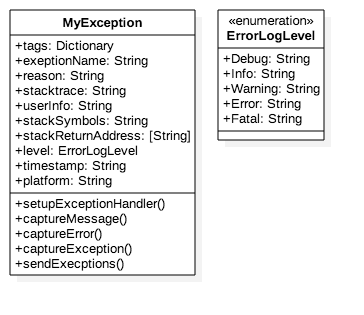
\includegraphics[width=100mm]{images/classdiagrams/Exception}
    \label{fig:exception-cd}
\end{figure}

\paragraph{Uncaught exceptions}

Uncaught exceptions makes the app crashes, so between the time crash happens and the app closes which is a small window, the exception has to be dealt with. Using the NSSetUncaughtExceptionHandler() with the parameter of function, that function is not allowed to make outside calls, which include HTTP request and function calls. So the exception is stored in UserDefaults which is a built in data dictionary that stores small amount of user settings for as long as the app is stored. When the user opens application again, the exception singleton class gets instantiated, and it does a check if any exceptions exists in UserDefaults, and then a HTTP post sends the exception to the server.

\paragraph{Caught exceptions}

Using the same class as above with uncaught exceptions, extra functionality was added to enable to developers to send these exceptions to the server. As the class is a singleton and gets initialized when the application opens, the sharedClient function can be used to return the instance of that object, then use the functions available to send the exceptions.
Some of these are shown in table \ref{table:exceptions}

\begin{table}[!h]
\centering
\caption{Caught Exceptions}
\label{table:exceptions}
\begin{tabular}{|c|l|l|l|}
\hline
\rowcolor{green!20}
\multicolumn{1}{|l|}{Library Method}                             & Description                                                                                            & \multicolumn{1}{l|}{Parameters}                                                                                                        & Result            \\ \hline
\begin{tabular}[c]{@{}c@{}}MyException.\\ sharedClient.\\ captureMessage();\end{tabular} & \begin{tabular}[c]{@{}l@{}}Captures the info message \\ and sends to the server\end{tabular}           & \begin{tabular}[c]{@{}c@{}}message : String,\\ method: String? = \#function, \\ file: String? = \#file, line: Int = \#line\end{tabular}                        & Successful/ Error \\ \hline
\begin{tabular}[c]{@{}c@{}}MyException.\\ sharedClient.\\ captureMessage();\end{tabular} & \begin{tabular}[c]{@{}l@{}}Captures the message\\  along with error level\\ to the server\end{tabular} & \begin{tabular}[c]{@{}c@{}}message: String, level: ErrorLogLevel, \\ method: String? = \#function , \\ file: String? = \#file, line: Int = \#line\end{tabular} & Successful/ Error \\ \hline
\begin{tabular}[c]{@{}c@{}}MyException.\\ sharedClient.\\ captureError();\end{tabular}   & \begin{tabular}[c]{@{}l@{}}Captures the error \\ and sends to the server\end{tabular}                  & \begin{tabular}[c]{@{}c@{}}error : NSError, method: String? = \#function,\\  file: String? = \#file, line: Int = \#line\end{tabular}                           & Successful/ Error \\ \hline
\end{tabular}
\end{table}


\section{Integrate into Live App}

For some parts of project, an already developed and published app called DIT-Timetable was used to add in the services, to test if Apple would allow it through. The services include remote configuration and language choice. Due to Apple's strict guidelines, the remote configuration was developed into the DIT-Timetable app into different phases, then each stage had a build and published.

\subsubsection{Phase 1}
This phase included just the basic remote configuration, with the capability of updating text such as page title, and label values. Apple did approve this phase, and while the app live, using the iPad prototyping app the text values were able to be changed. 

\subsubsection{Phase 2}

Phase 2 gave the ability to adjust user interface values such as text colour, text size and user interaction enabling/disabling. This also been approved by Apple giving it a go ahead to be completely integrated into the project.

\subsubsection{Phase 3}

\section{Dashboard Development}

The dashboard was originally going to be created as an iPad app, but after some thought that not all mobile developers can be expected to own an iPad, the dashboard was developed as a Mac App. In the design chapter, the layout and design of the dashboard was discussed including what functionality will be provided to the developers.

Mac Application using Swift 2 was used to develop the user interface that will enabled the developer to configuration their mobile backend.

\subsection{Project structure}

Xcode IDE was used to develop the dashboard interface with help of libraries. These libraries included Cocoa(API) and Charts. Cocoa is Apple's native object-oriented application programming interface (API) for their operating system macOS. The cocoa consists of the Foundation Kit, Application Kit and Core Data frameworks. It is responsible for the appearance of apps and their responsiveness to user actions. The figure illustrates where the Cocoa frameworks resides. Charts is a third party framework provided by developer called Daniel Cohen Gindi that can be found on Github. \cite{charts} 

Already discussed in the design chapter, Apple gives an extensive section on Human Interface Guidelines on which to follow when developing Mac applications. So following these guidelines will help develop an application that can be submitted to the Mac App store. The IDE that will be used as already stated is Xcode, inside Xcode their are a number of views that can be used. In the following sections, the two main areas which will be mentioned are Interface builder and Code Editor views. The Interface Builder is where the storyboards can be edited. They are an user interface way of designing and developing the UI of an application, and the code editor view is what connects the UI view to the class files.

\begin{figure}[!h]
    \caption{Cocoa \cite{cocoa}}
    \centering
    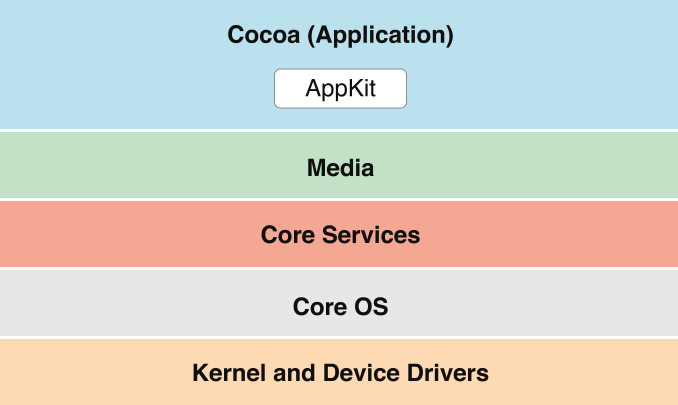
\includegraphics[width=75mm]{images/dashboard/cocoa}
    \label{fig:apns}
\end{figure}

\subsection{Dashboard Views}

\subsubsection{Login view}

\begin{figure}[!h]
    \caption{Log in class diagram}
    \centering
    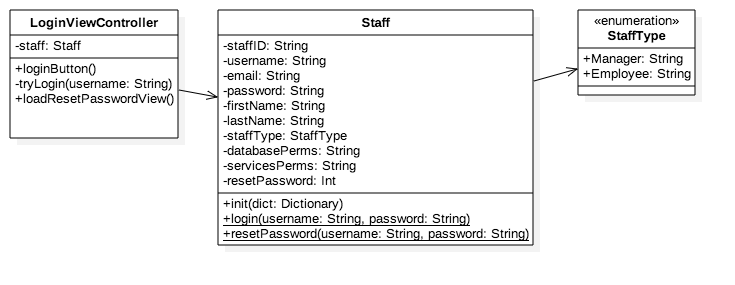
\includegraphics[width=150mm]{images/classdiagrams/Login}
    \label{fig:login_cd}
\end{figure}

Figure \ref{fig:login_cd} illustrates the class diagram for the main view controller for the log in view, as well as the staff object that were used to authenticate the user. 

In figure \ref{fig:log-in-view} illustrates the dashboard simple sign in view where the user gets verify with their credentials. The view contains three input values which the user must put in, as the server can be deployed on any server, the user is asked to put in the IP or domain name where the server is located. The other two values is user-name and password, and then there is option for the user to tick the remind me box, which keeps the user logged in. The Log-in button sends POST request to the server along with both values. A register button was decided against, as this is a restrictive application. The administrator once logged in, can create new users explained later on.

\begin{figure}[!h]
    \caption{Log-in View}
    \centering
    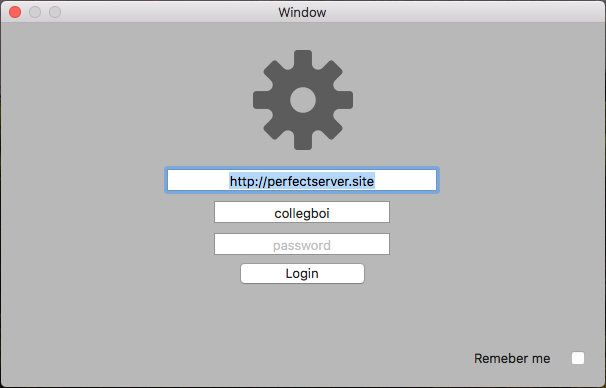
\includegraphics[width=75mm]{images/dashboard/login}
    \label{fig:log-in-view}
\end{figure}

\newpage
\subsubsection{Menu}

% \begin{figure}[!h]
%     \caption{Menu}
%     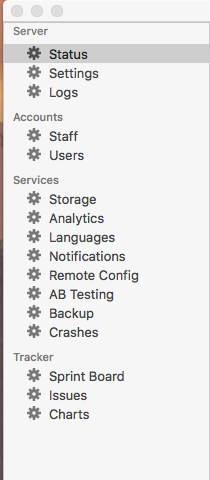
\includegraphics[width=50mm]{images/dashboard/menu}
%     \label{fig:menu}
% \end{figure}

% \begin{wrapfigure}{r}{0.25\textwidth} %this figure will be at the right
%     \caption{Menu}
%     \centering
%     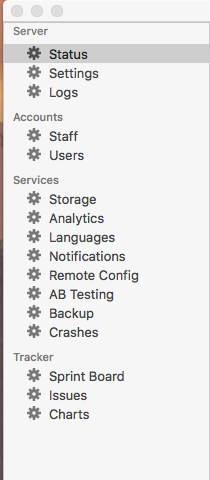
\includegraphics[width=0.25\textwidth]{images/dashboard/menu}
%     \label{fig:menu}
% \end{wrapfigure}

Figure \ref{fig:menu} illustrates the side bar navigation. This routes the user across the whole application.

\subsubsection{Status}

\begin{figure}[!h]
    \caption{Status View}
    \centering
    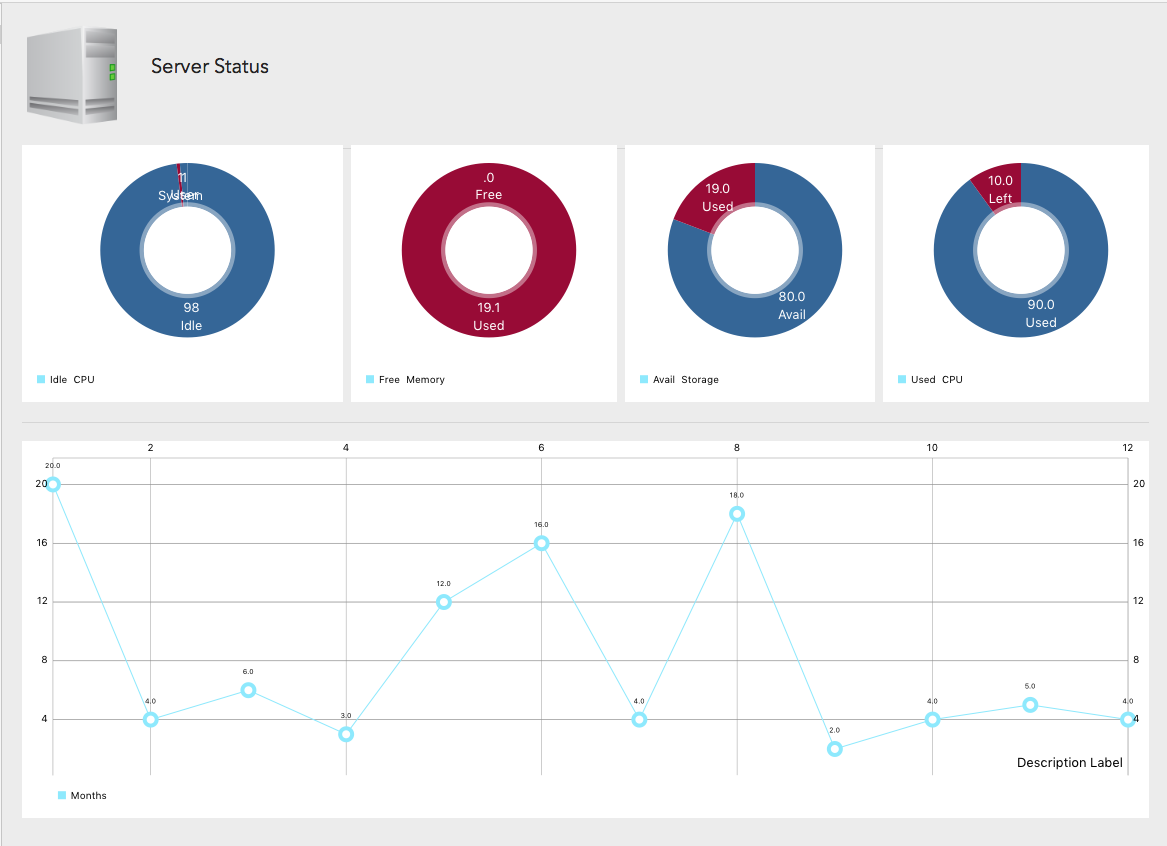
\includegraphics[width=100mm]{images/dashboard/status}
    \label{fig:status-view}
\end{figure}

Figure \ref{fig:status-view} illustrated the server status view, it is the first page the user sees when entering the application. This view displays a number of graphs about the server. To help with displaying graphs, a framework was used called Charts, and figure \ref{lst:pie-chart} illustrates the code necessary to display a pie chart. 

Starting from left to right with the pie charts, the first displays the current CPU usage, next storage usage and memory usage. The line chart displays the history and current CPU usage. This gives the developer an general overview on what the physical sever doing. This can help decide whether or not to upgrade the system.

\lstinputlisting[label={lst:pie-chart},language=Swift, caption=Pie Chart]{development/code/piechart.m}

\subsubsection{Settings}

\begin{figure}[!h]
    \caption{Settings View}
    \centering
    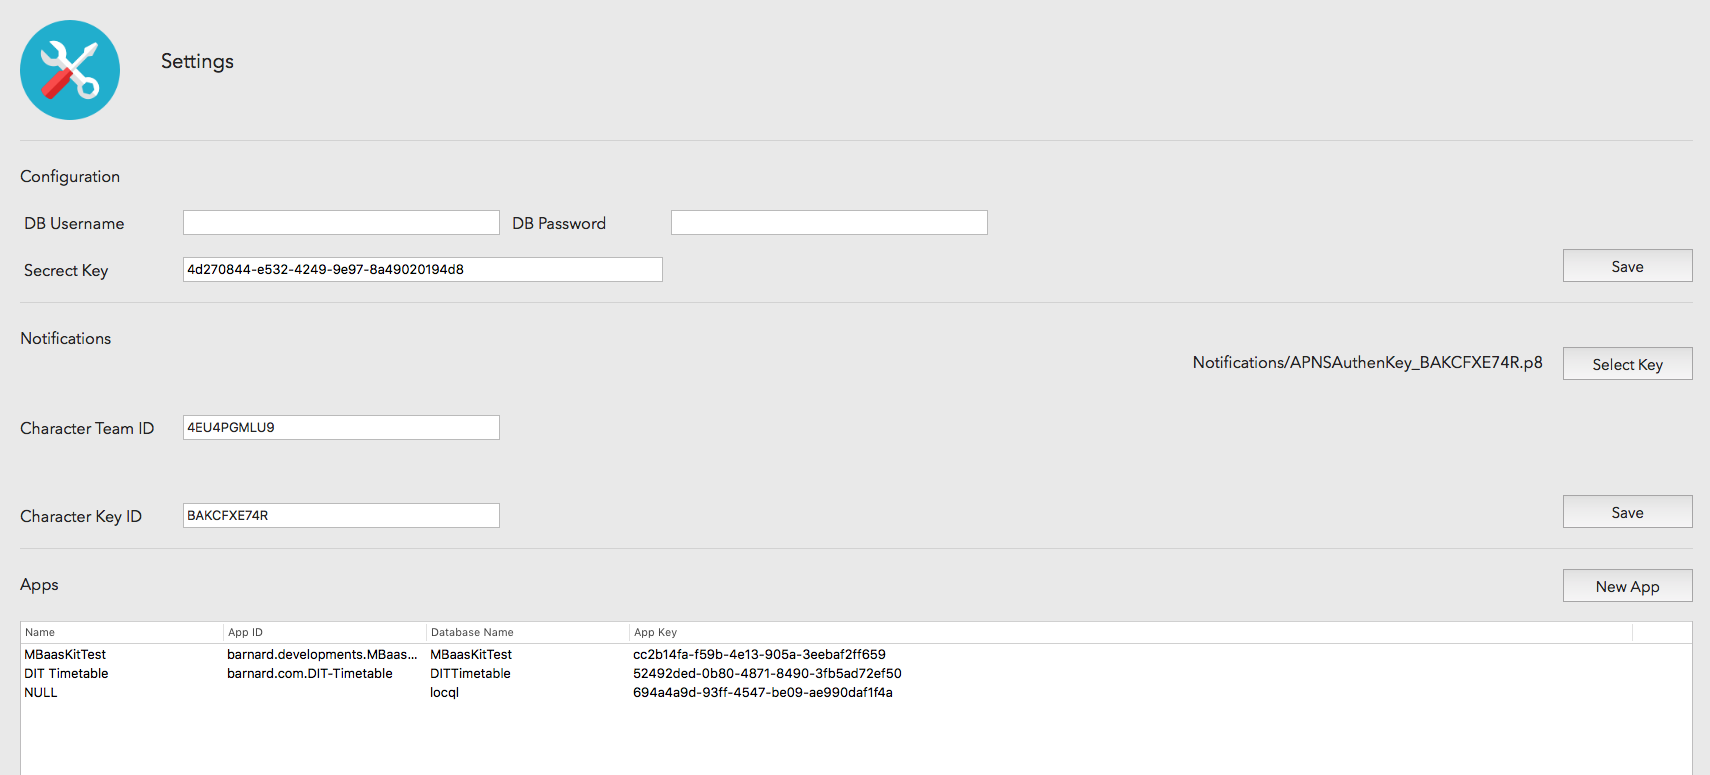
\includegraphics[width=150mm]{images/dashboard/settings}
    \label{fig:settings-view}
\end{figure} 


\begin{figure}[!h]
    \caption{Apps Class Diagram}
    \centering
    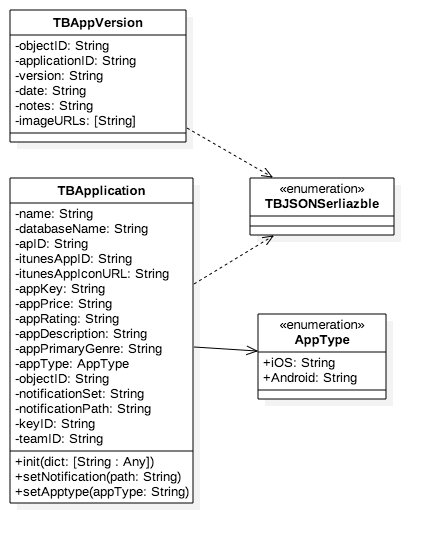
\includegraphics[width=75mm]{images/classdiagrams/Settings}
    \label{fig:settings-cd}
\end{figure} 

Figure \ref{fig:settings-view} illustrates the settings view, where the configuration for the web-server and the mobile applications. The view is split up into three sections, the first section has some configurations values for accessing the web-server and database. The secret key, is part allows the mobile applications to access the web-server. This key is added to each request made to the API. The database user-name and password can be set, and allows for some extra security.

The notification section is for configuring the Apple Push Notifications (APNs), this has changed in the past year was mention in the design chapter. The process now has sped up how to set up the APNs on both the Apple developer console and the server. Now one key file with extension .p8 is all that is required to send APNs, this and three other values are required. Two of them are the team id, which is the developers id found in the developer console, and the key id which is provided when requesting a new .p8 key file. The Select Key buttons brings up file window, to get the file from the developers computer, and uploads the file via HTTP to the server. Once the Save button has been selected, the three values are sent to the database.

\begin{figure}[!h]
    \begin{subfigure}{0.5\textwidth}
        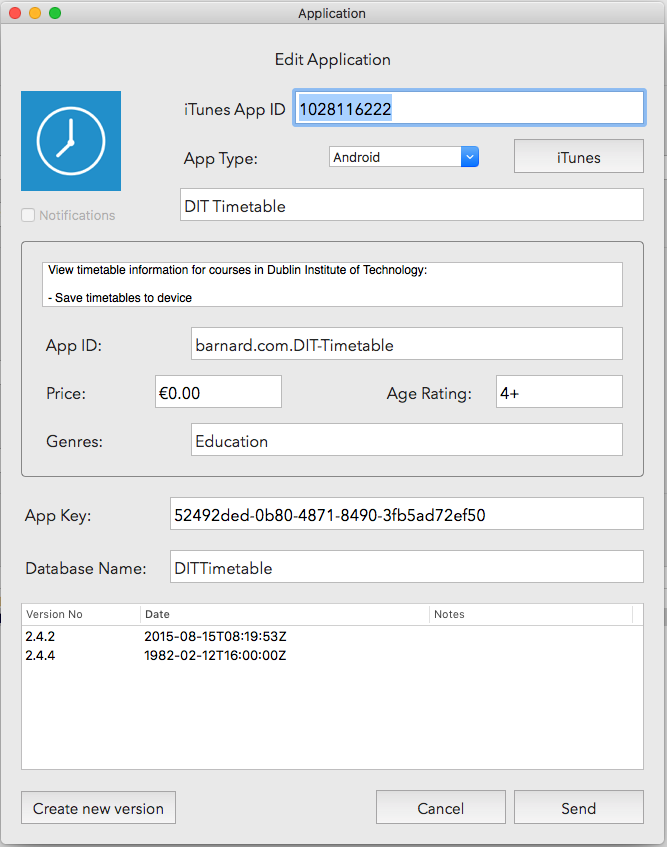
\includegraphics[width=0.9\linewidth, height=10cm]{images/dashboard/newapp}
        \caption{App View}
        \label{fig:subim1}
    \end{subfigure}
    \begin{subfigure}{0.5\textwidth}
        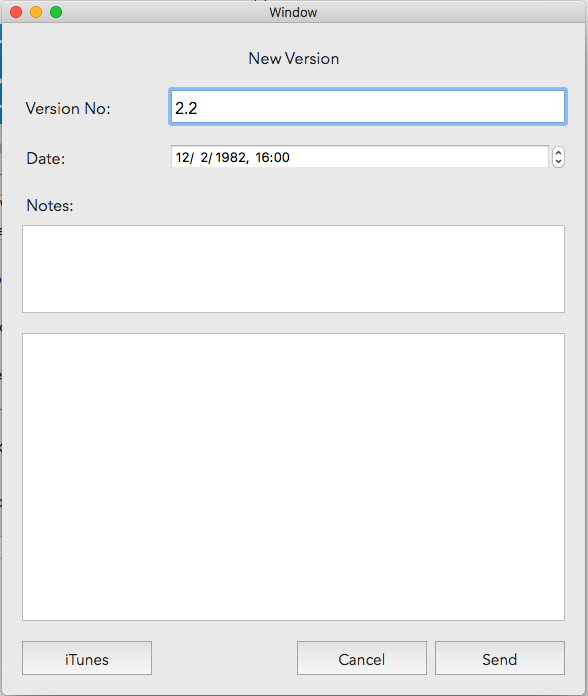
\includegraphics[width=0.9\linewidth, height=10cm]{images/dashboard/newversion}
        \caption{App Version}
        \label{fig:subim2}
    \end{subfigure}
\caption{Configuring Apps}
\label{fig:app-version}
\end{figure}

\begin{figure}[!h]
    \caption{iTunes API}
    \centering
    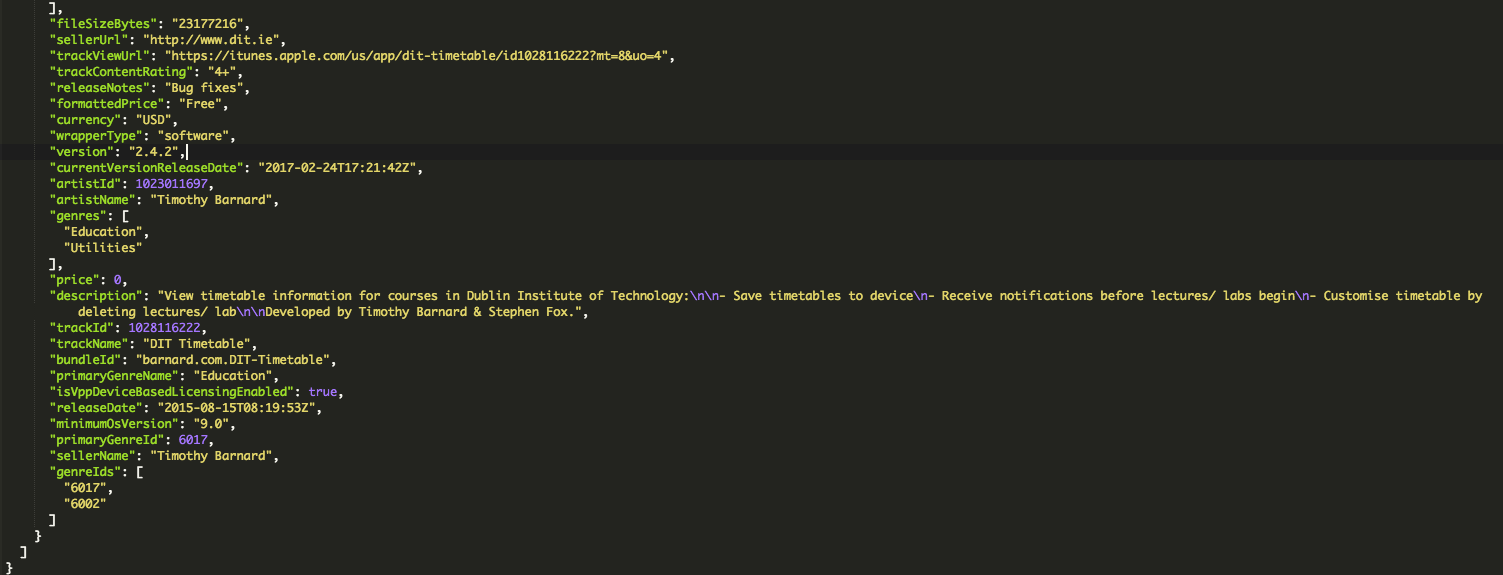
\includegraphics[width=150mm]{images/itunes-api}
    \label{fig:itunes-API}
\end{figure} 

Figure \ref{fig:settings-cd} illustrates the classes for the application and version, and Figures \ref{fig:app-version} shows where these values are displayed. Each application contains a number of properties, and some of these are provided by Apples app API. In figure \ref{fig:subim1}, the button iTunes once the user has entered the iTunes App ID field retrieves a number of values which are displayed inside the box along with the app icon. The URL for making the request is https://itunes.apple.com/lookup?id=, and the app id is passed into the GET request, and JSON objects are returned to be parsed into objects as seen in figure \ref{fig:itunes-API}. After being parsed into iTunes object, these are then set into the TBApplication class to be saved in the database.

This can only be done once the application has been published, but the other fields can be entered until then. The two important fields from this view is app key and database name, these are a security feature. Each applications gets their own database, by doing this keeps the data separate from other applications. The second security feature is the app key, this provides access to the applications database. As mentioned in the settings section, the secret is sent up each request, this is also the same with the app key. This will be discussed more in the server section later. 

In figure \ref{fig:subim2}, the developer can keep history of app versions published. The iTunes API already mentioned does not provided history of published version, so by having the feature gives the developer a history of what changes has been made in each version. This view also displays any notes and app stores images that have been added in that version. The iTunes button at the bottom left, does the same as in figure \ref{fig:subim1}, but this view retrieves different fields to be save. The reason for this button, is that when a new version is published, the app id will return the new app versions data only.


% \begin{figure}[!h]
%     \caption{App View}
%     \centering
%     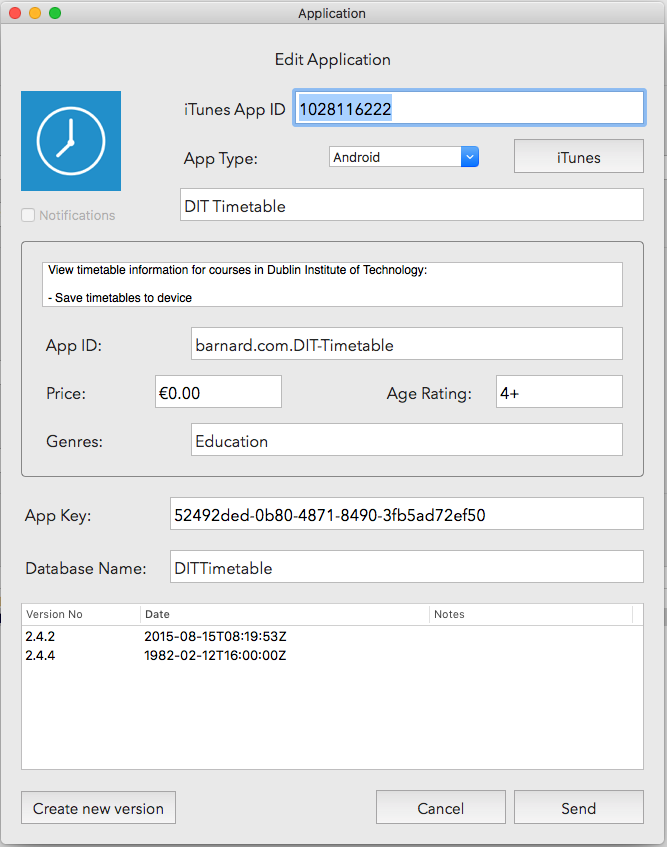
\includegraphics[width=75mm]{images/dashboard/newapp}
%     \label{fig:newapp-view}
% \end{figure}  

% \begin{figure}[!h]
%     \caption{App Version View}
%     \centering
%     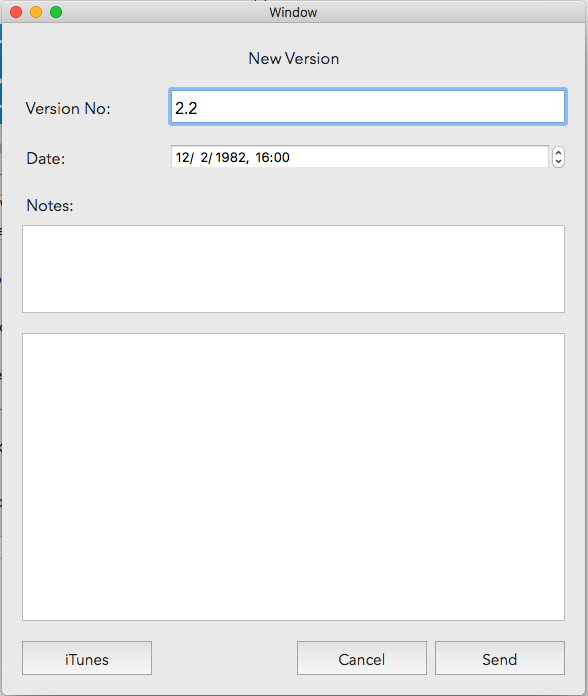
\includegraphics[width=75mm]{images/dashboard/newversion}
%     \label{fig:newversion-view}
% \end{figure}  

\subsubsection{Logs}

\subsubsection{Admin}

\subsubsection{Storage}

\subsubsection{Analytics}

\subsubsection{Languages}

\subsubsection{Notifications}

\subsubsection{Remote Configuration}

\begin{figure}[!h]
    \caption{Remote Configuration View}
    \centering
    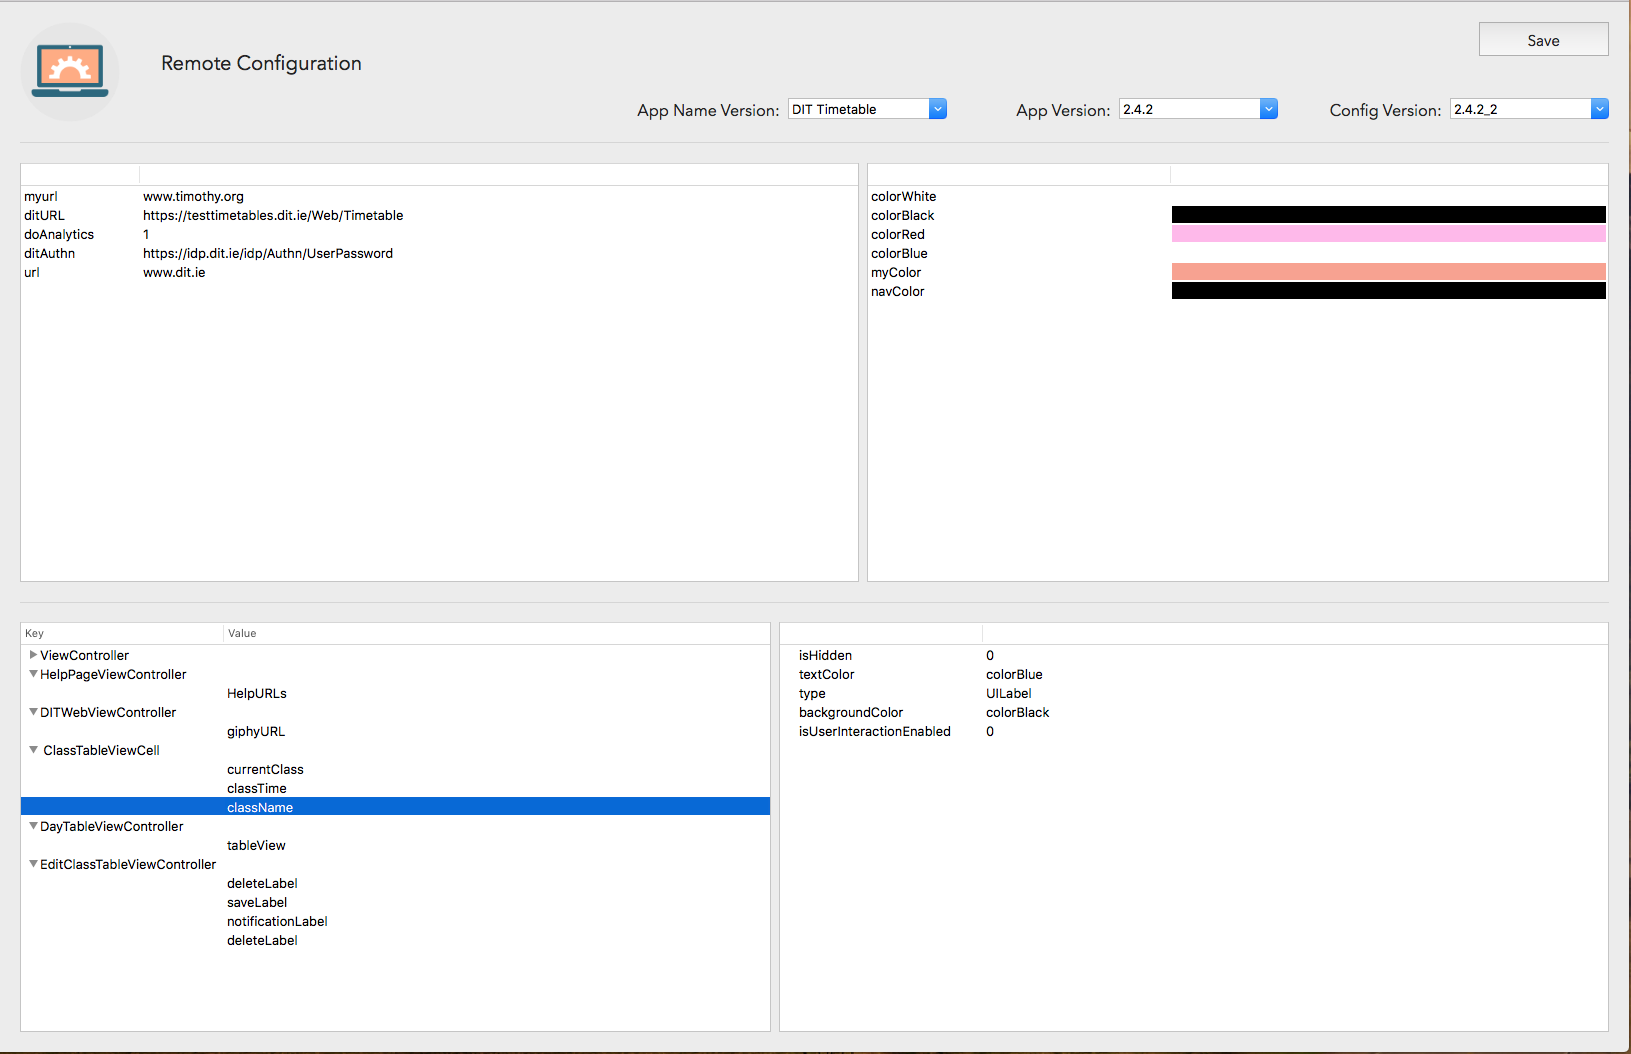
\includegraphics[width=150mm]{images/dashboard/remote-config}
    \label{fig:remote-config-view}
\end{figure}

\begin{figure}[!h]
    \caption{Remote Configuration View}
    \centering
    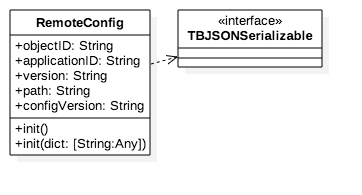
\includegraphics[width=80mm]{images/classdiagrams/RemoteConfig}
    \label{fig:remote-config-cd}
\end{figure} 

The remote configuration view as illustrated in figure \ref{fig:remote-config-view} contains four tables which in turn represents the four classes already discussed in the services section \ref{fig:rc-cd}. The figure displays the current configuration for the DIT-Timetable app with version 2.4.2. When the page initially loads, the first of each drop down list to display that current configuration. The first of the drop down menus display the list of applications, which are taken from TBApplication collection. This collection are set from the settings view already discussed, along with the applications versions, which is the contents of the next drop down. The last list contains the current configuration versions as seen in table \ref{fig:remote-config-cd}. Each remote configuration object has an application and version, its relates to. The configVersion property allows A/B Testing which be discussed next to use. 

Starting from the top left table which contains the main settings values, next on the right at the colours used in that particular version in the app. The bottom left table contains the view controller or classes, and if a class contains objects the cell can be expanded to display all the objects. Once an object has been selected, the table on right contains all possible properties that can be used. This part of the dashboard also contains a JSON file, that contains all UI objects that can selected with their properties as illustrated in listing \ref{lst:label_json}. If a property options are a list type, then the raw string values are shown, for example textAlignment. In Swift, the UI object property options are type of enumeration, so when the user chooses an option the integer value is stored. When an property has been selected, ethier two of views will show as illustrated in figure \ref{fig:property1}. The value can then selected and set.

\lstinputlisting[label={lst:label_json}, caption=UI Object JSON]{development/code/Label_json.m}

\begin{figure}[!h]
    \caption{Edit Property View}
    \centering
    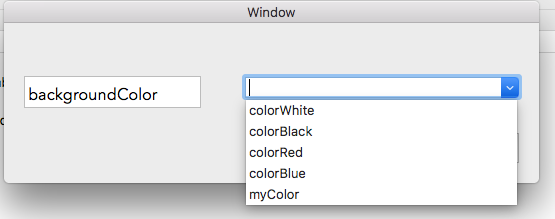
\includegraphics[width=80mm]{images/dashboard/property-1}
    \label{fig:property1}
\end{figure} 

\begin{figure}[!h]
    \caption{Save Configuration View}
    \centering
    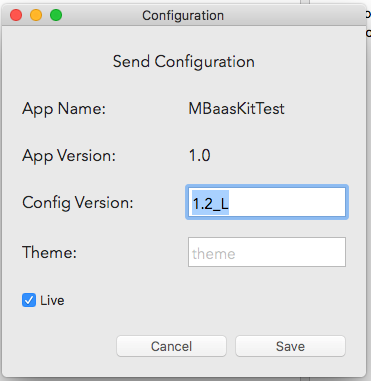
\includegraphics[width=80mm]{images/dashboard/configuration}
    \label{fig:configuration}
\end{figure} 

Once the configuration has been set, the user has the option to save and publish that version. This can be done by pressing the Save button at the top right which displays a new window as illustrated in \ref{fig:configuration}. This view allows the user to set the version name and theme. This theme then can be used in the application for the mobile end user to choose. This will be illustrated later in the testing chapter. The live check box if unchecked can restrict this version for the mobile application to use. 

\subsubsection{AB Testing}

\begin{figure}[!h]
    \caption{AB Testing View}
    \centering
    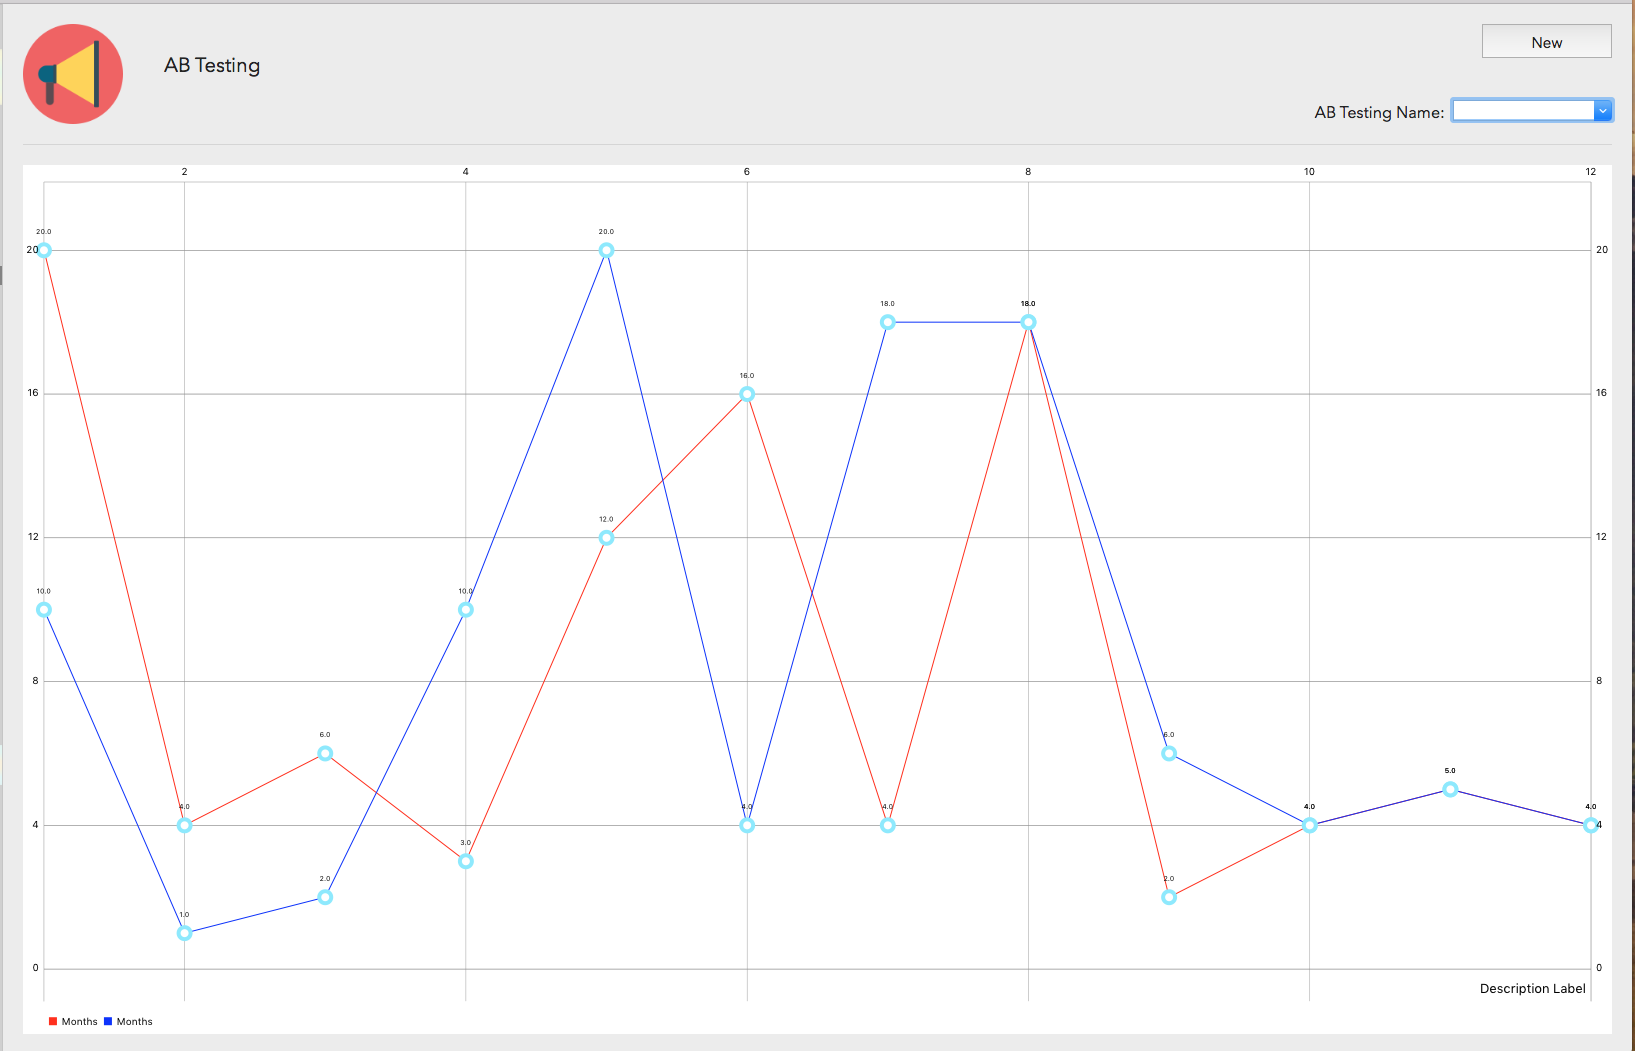
\includegraphics[width=120mm]{images/dashboard/abtesting}
    \label{fig:abtesting-view}
\end{figure} 

\begin{figure}[!h]
    \caption{AB Testing Config View}
    \centering
    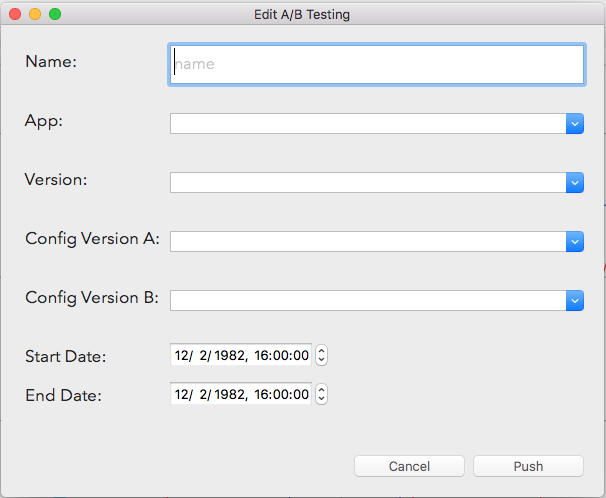
\includegraphics[width=100mm]{images/dashboard/abtesting-config}
    \label{fig:abtesting-config-view}
\end{figure} 

Figure \ref{fig:abtesting-view} illustrates the AB Testing view, and figure \ref{fig:abtesting-config-view} shows how to configure the AB Testing object. The main AB testing view displays a line chart with two line. Each line corresponds to a version that has been include that a particular testing set up as was already discussed with figure \ref{fig:abtesting-cd}. The analytical data gathered is from the TBAnalytics class that was discussed in section Analytics.

The drop down list can used to select a particular testing, and then can be view to see what configuration version had the highest usage. To configure a new A/B testing, the new button is pressed to display the new in figure \ref{fig:abtesting-config-view}. The following values are required to be set, the name, the application name, the particular version of the app and the next two drop down list are the different versions that was already configured in Remote Configuration view. The start and end time are set to allow a time frame for which these test are run. Once all the values have been entered, the push button will send the new object to the database, and when a request is made to server for a configuration file, the ab testing object will be retrieved and one of the versions will be shown. This will be discussed more in the web-server section.

\subsubsection{Backup}

\subsubsection{Crashes}

\begin{figure}[!h]
    \caption{Crashes View}
    \centering
    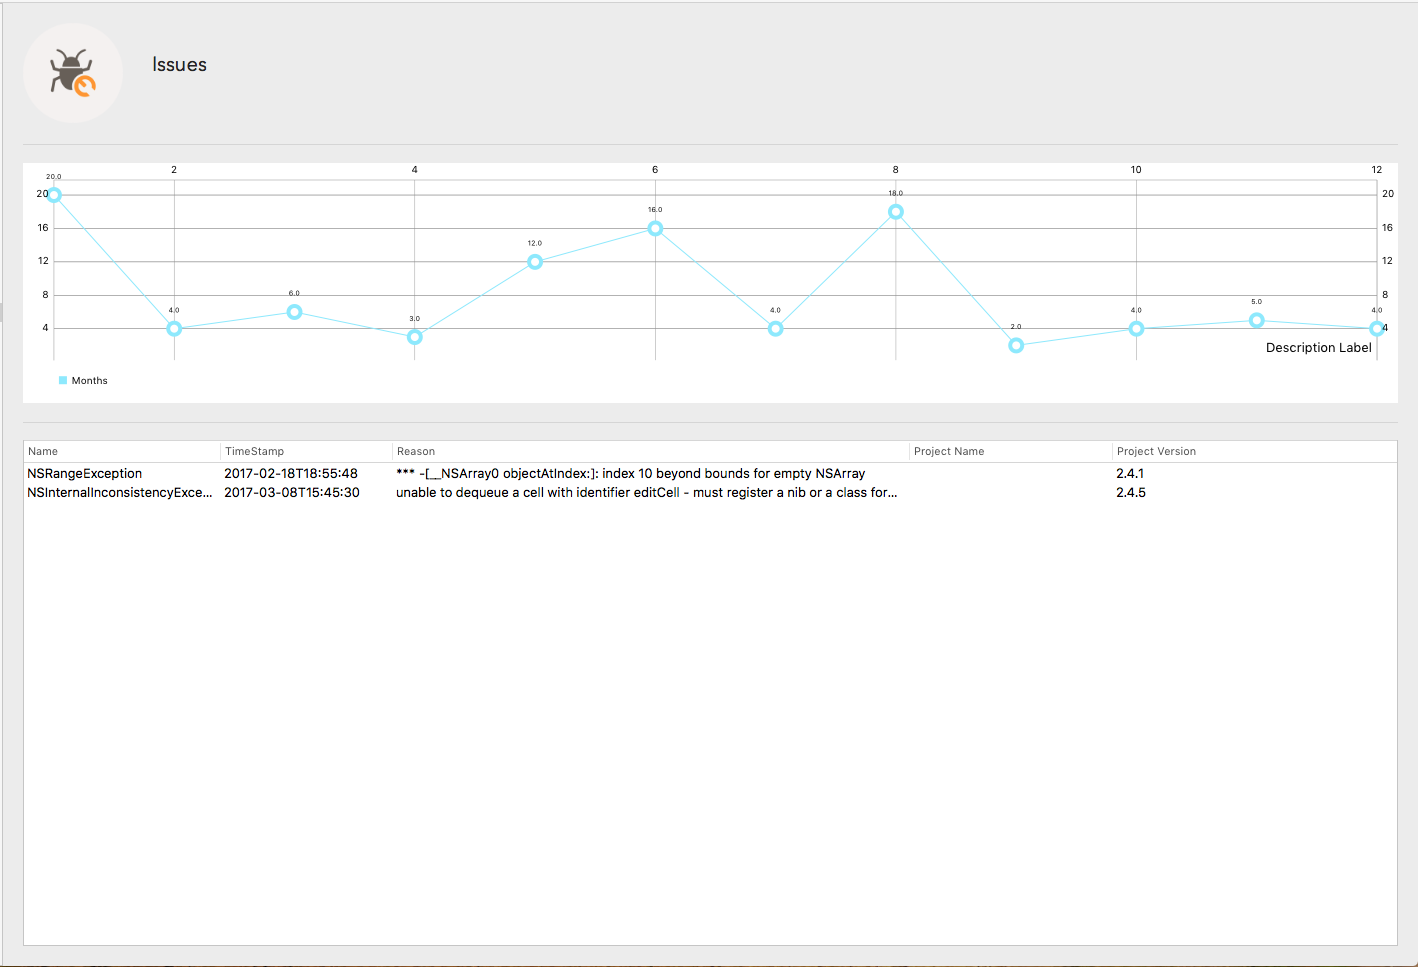
\includegraphics[width=150mm]{images/dashboard/crashes}
    \label{fig:crashes-view}
\end{figure} 

\subsubsection{Tickets}

\begin{figure}[!h]
    \caption{Tickets View}
    \centering
    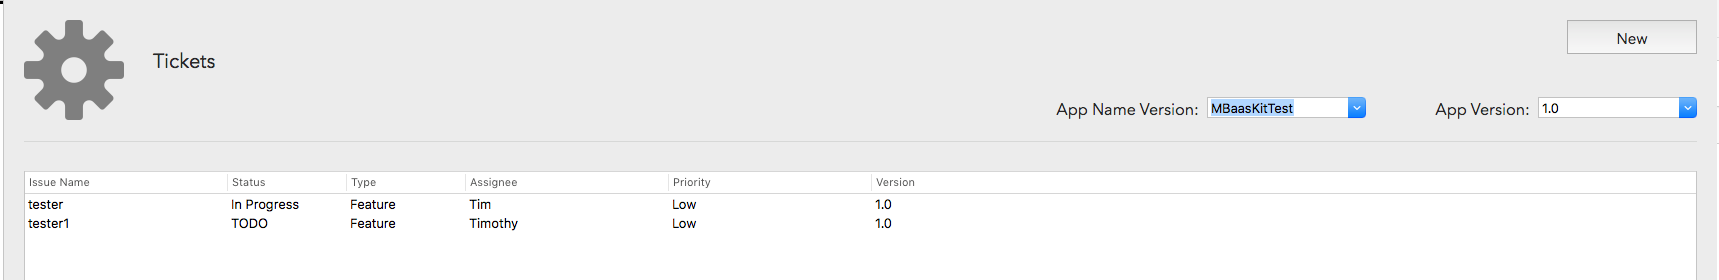
\includegraphics[width=150mm]{images/dashboard/tickets}
    \label{fig:issues-view}
\end{figure} 


\begin{figure}[!h]
    \caption{Issues Class Diagram}
    \centering
    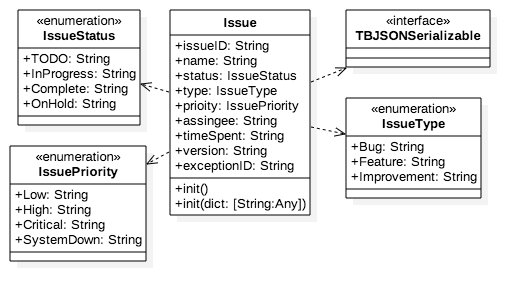
\includegraphics[width=100mm]{images/classdiagrams/Issues}
    \label{fig:issues-cd}
\end{figure} 

Figure \ref{fig:issues-view} illustrates the tickets view page containing all different type of tickets being, bugs, features etc are displayed. After selecting the application name and version from the drop down list, the table below will get populated with the current issues relating to that application. The class diagram for each issue is illustrated in figure \ref{fig:issues-cd}, where the Issue class has the same protocol again. This give the class functionality to save and retrieve all the issues. The issue class consists of few enumeration type variables, where issue can be a bug, the issue has a status and priority. A enumeration was used to make sure of the value being parsed into the database, being only one of the values.

To be able to create a new issue, a new window was developed. This view as seen in figure \ref{fig:new-issue}.

\subsubsection{Sprint Board}

\begin{figure}[!h]
    \caption{Sprint Board View}
    \centering
    \includegraphics[width=150mm]{images/dashboard/sprint-board}
    \label{fig:sprint-board-view}
\end{figure} 

Figure \ref{fig:sprint-board-view} illustrates the sprint board view, where the tickets/issues from the previous section will show. This view gives the developer an easier layout to monitor when working through assigned tickets. The issues can also be dragged and moved into a different table, so moving an issue from in progress section to completed. The main function for this can be seen in listing \ref{lst:sprint}, which looks after moving the value into the correct table.

\lstinputlisting[label={lst:sprint},language=Swift, caption=Sprint]{development/code/sprint.m}

\section{CocoaPod Framework}

First the CocoaPod was initialised, and this was done all in command line as see in listing \ref{lst:pod_init}. The first command installs CocoaPods, then once that was installed, the pod was created. The pod lib lint creates the skeleton structure and associated files, next to create the project, pod lib create MBaaSKit was run which was followed by terminal asking for a number of inputs.

\lstinputlisting[label={lst:pod_init}, language=Bash, caption=Pod Init]{development/code/pod_init.m}

\begin{itemize}
  \item What language do you want to use?
  - Swift
  \item Do you want to include demo application?
  - Yes
  \item What testing framework do you use?
  - None (this will be done later)
  \item Do you want to view based testing?
  - No
\end{itemize}

After the pod is initialised, the .podspec files needs to be updated, so running nano MBaaSKit.podspec to edit the file. The following values are required to be updated: 

\begin{itemize}
  \item s.summary
  - a brief summary of the pod
  \item s.description
  - a brief description of the pod
  \item s.homepage
  - Github link to the location of the pod
\end{itemize}

After the pod has been setup, the next listing \ref{lst:pod_git} adds all the files, and commits to local origin repository and pushes to master.

\lstinputlisting[label={lst:pod_git}, language=Bash, caption=Pod Github]{development/code/pod_git.m}

At this stage the pod has been set up, and the initial Github commit has been pushed. 

Once the project files and code has added, the next stage was to make the pod available known as pod tagging. This was done by running the following commands in listing \ref{lst:pod_tagging}. The first command git tag "0.0.1" was run, which gives a version, then git push origin "0.0.1". After which pod spec lint MBaaSKit.podspec verifies that everything is configured correctly between where the source code is stored and the .podspec file. The output states "MBaaSKit.podspec passed validation", so the last command to push the pod can be done. 

\lstinputlisting[label={lst:pod_tagging}, language=Bash, caption=Pod Tagging]{development/code/pod_tagging.m}

\section{Web-server}

The web server developed was split up into two sections; the development of the web-server using the framework Perfect and setting up the server, and creating the installation file which will installed all the required dependency packages.

\subsubsection{Deployment}

DigitalOcean was used as server of choice and to create a virtual private servers or as DigitalOcean calls them Droplets. After creating an account and going to the page to create a droplet, the first choice was of distribution. The project required Ubuntu 16.04, after which the droplet size was asked, as for this project the basic 512MB ram, 20GB SSD Disk and 1000 GB transfer package was chosen. The next option was what region the droplet will be located and decided to go with London being the closest. Step 5 was additional options where IPv6 was chosen, for Apples requires the server to contain both IPv4 and IPv6. Step 6 was setting up SSH keys, which was done, and the last step was to give the droplet a name for the dashboard purposes.

After the droplet had been created and to log in from the computer, terminal was used with the following command: ssh root@p<droplet ip address>. Once the password had been entered, a prompt message asking to set up SSH keys and followed by entering YES. After logging in a number of steps to setup and install the required packages, while running these commands and checking they installed correctly, they were added to a script file which would be used to create the installation script.

\paragraph{Step 1}
The first step once logged in, was to create a new user and password for security purposes. This was done by running the following commands in listing \ref{lst:username}.

\lstinputlisting[label={lst:username}, language=Bash, caption=Setting user-name]{development/code/username.m}

\paragraph{Step 2}
Next the server required to set the locale along with updating and upgrading.
\lstinputlisting[label={lst:init_server}, language=Bash, caption=Updating Server]{development/code/init_server.m}


\subsubsection{Development}

To start developing the server, Perfect provides a basic template with just the structure to start off with, found at https://github.com/PerfectlySoft/PerfectTemplate. A new directory was created, then running the command git clone following https://github.com/PerfectlySoft/PerfectTemplate.git. One the template was download, running the following command would create an Xcode project: swift package generate-xcodeproj. The package.swift file required updating with the required packages such as MongoDB and Notifications etc, then running the command sudo swift build inside the project directory retrieved all the packages that was included in the package.swift file. The project structure contains sources and packages directories, the packages are which was already downloaded and the sources where the web-server files are placed. 

The web-server starts off with the main.swift which includes the creation the HTTP server, and adding routes and setting the port number, then starting the server. The routes are where each REST request will go, so for example if request /user then the route will go to the user class. An example of the routes is shown in listing \ref{lst:routes}. This example is the routes for the database, retrieving and sending object. The function is called from the main.swift file, which returns all the routes for the database handler class. The handler parameter is the method name in the same class for which implementation is done depending on the route.

\lstinputlisting[label={lst:routes},language=Swift, caption=Routes]{development/code/routes.m}

\section{Code Stats}

\begin{table}[!h]
\centering
\caption{Project Code Stats}
\label{my-label}
\begin{tabular}{|l|l|l|}
\hline
\rowcolor{green!20}
Deliverable & Files & Code   \\ \hline
Server      & 33    & 2,663  \\ \hline
Dashboard   & 264   & 27,507 \\ \hline
SDK         & 36    & 2,271  \\ \hline
Total       & 333   & 29,778 \\ \hline
\end{tabular}
\end{table}
\chapter{Implementation}


\section{Installation Deployment}

One of the key components of my project is the back-end web application. As one of services I am providing is self hosted. So developer can host their own back-end on any server of their choosing as long as the operating system is Ubuntu 16.04. The complete system is available on Github.

\url{https://github.com/collegboi/PerfectServer}

\lstinputlisting[label={lst:login}, language=Bash, caption=Server Login]{implementation/code/login.m}

SSH, or secure shell is a network protocol that provides a secure, encrypted way to communicate with your server. In Figure \ref{lst:login} is used to log in to your server. The user-name by default by root but we will change this next and the next field is the IP address of your server.


\lstinputlisting[label={lst:user-name}, language=Bash, caption=Setting user-name]{implementation/code/setting-username.m}

 In Figure \ref{lst:user-name} we are going to set your new user-name and password. Doing this will help secure your server by moving away from the default root user-name.

\lstinputlisting[label={lst:github}, language=Bash, caption=Installing]{implementation/code/github.m}
Last is to pull down the server from Github and install all the necessary packages This is done by running the following commands one at a time in Figure \ref{lst:github}.


\section{Development}

\subsection{Add the SDK}

\lstinputlisting[label={lst:pod_init},language=Bash, caption=Init pods]{implementation/code/pod_init.m}

After creating if you don't have an Xcode project, you will want to install the SDK. This will be done using CocoaPods. CocoaPods is a dependency manager for Swift projects. It contains thousands of libraries that can be used in your apps. One of which is MBaasKit. Start off with stepping into your project as seen in Figure \ref{lst:pod_init}.

Next we will add the MBaasKit pod to the file \ref{lst:pod}.

\lstinputlisting[label={lst:pod},language=Bash, caption=Pod file]{implementation/code/pod.m}

Last part for adding the SDK to your project is to install the pod. This can be done by running the command in Figure \ref{lst:pod_install}

\lstinputlisting[label={lst:pod_install},language=Bash, caption=Pod install]{implementation/code/pod_install.m}

\subsection{Using the SDK}

Once the SDK has been included in the project, the following values are required to be added in the Info.plist file.

\begin{enumerate}
  \item APPKEY - from the dashboard settings view, in the application window
  \item SERVERKEY - the secret key in the dashboard settings view
  \item URL - the domain name for the location of the web server
\end{enumerate}

\subsubsection{Remote Configuration}

Remote Configuration provides the ability to maintain the application user interface in production. The framework contains a list of protocols for the UI objects such as UITextField, UITableView etc. This protocol will grab the required properties for the object from locally stored configuration files. This files are download initially when the application is first opened, and the end user has the option depending on the developers choice of themes if any. The steps required to implement this is shown in the following listing \ref{lst:rc}.

\lstinputlisting[label={lst:rc},language=Swift, caption=Remote Configuration Setup]{implementation/swift/rc_implemented.m}

To handle downloading a new theme that the end user can select, the listing \ref{lst:new_theme} illustrates how this is done. The call back function takes the parameter of the theme name, once the call back has been called, updating the view can be done. Line 4 is update the configuration file with the reading file name. This can be changed to be included in function that handles when the app goes in the background. The updateViews() function can be implemented to refresh the view if changes are immediate.

\lstinputlisting[label={lst:new_theme},language=Swift, caption=Retrieving new theme]{implementation/swift/config_update.m}

\subsubsection{Notifications}
To start using notifications, we first need to create the installation object and send that to our server. This is done by adding the following function \ref{lst:installation} in our AppDelegate file.

\lstinputlisting[label={lst:installation},language=Swift, caption=Register for Notifications]{implementation/swift/installation.m}

\subsubsection{Storage}

\lstinputlisting[label={lst:object},language=Swift, caption=Storing/Retrieving Objects]{implementation/swift/object.m}

As you can see in Figure \ref{lst:object}, when creating a struct and using the protocol JSONSerialiszable, we can then send and retrieve the objects in the backgrounds using those commands.


\subsubsection{Exception Handling}

Exception is a problem that arises during the execution of a program. If exceptions are not handled, it can cause the app to crashes and when the app is live, we would have no way of knowing. But by adding the following lines 1 and 2 in Figure \ref{lst:exception} we can catch uncaught exceptions and send them to our back-end storage and view with the dashboard. Line 4 is an example of sending a caught exception that can have a message sent along.

\lstinputlisting[label={lst:exception},language=Swift, caption=Storing/Retrieving Objects]{implementation/swift/exception.m}
\chapter{Testing and Evaluation}

\section{Testing}

Software testing is an investigation conducted to provide information about the quality of the product or service under test. Testing is executing a system in order to identify any gaps, errors, or missing requirements in contrary to the actual requirements. In my project I am using test-driven approach method, this helps eliminate parts of the code that will not work or fix them before adding them to system.

\subsection{Service testing}

As this project is Test Driven Development approach, all service unit testing has previously been done. These tests were done by building a small client application in Playground and web-server in Perfect which was developed and ran in Xcode. The API requests were tested afterwards using the Postman application, to run each API request and ensure the result is as expected. The tested included check the secret key and application key were authenticated, and if an incorrect key was used, then an error would be returned. Included bottom are some of the requests made along with the response in table \ref{tb:service-testing}.

\begin{table}[!h]
\centering
\caption{Service Testing}
\label{tb:service-testing}
\begin{tabular}{|c|c|c|l|l|}
\hline
\rowcolor{green!20}
\multicolumn{1}{|l|}{API Call}  & \multicolumn{1}{l|}{HTTP method} & \multicolumn{1}{l|}{Response}   & Body    & Result \\ \hline
\begin{tabular}[c]{@{}c@{}}http://perfectserver.site/api/\\ cc2b14fa-f59b-4e13-905a-3eebaf2ff659/\\ storage/RemoteConfig\end{tabular} & GET                                                      & Figure \ref{fig:api1}                                                                                                            &                                                                                                                                                     & PASS                           \\ \hline
\begin{tabular}[c]{@{}c@{}}http://perfectserver.site/\\ storage/TBAnalyitcs/\end{tabular}                                             & GET                                                      & \begin{tabular}[c]{@{}c@{}}\{,"result": "error"\\ ,"message": ""\}\end{tabular}                                             &                                                                                                                                                     & FAIL                           \\ \hline
\begin{tabular}[c]{@{}c@{}}http://perfectserver.site/api/\\ cc2b14fa-f59b-4e13-905a-3eebaf2ff659/\\ storage/Friends\end{tabular}      & GET                                                      & Figure \ref{fig:api2}                                                                                                            &                                                                                                                                                     & PASS                           \\ \hline
\begin{tabular}[c]{@{}c@{}}http://perfectserver.site/api/\\ cc2b14fa-f59b-4e13-905a-3eebaf2ff659/\\ storage/Friends\end{tabular}      & POST                                                     & \begin{tabular}[c]{@{}c@{}}\{,"result": "success",\\ "message":\\  "0e9635f6-b3fd-408d-\\ b4a2-458dab34c781"\}\end{tabular} & \begin{tabular}[c]{@{}l@{}}\{"dob": "12/12/2016",\\ "age": "44",\\ "name": "Jimmy"\\ ,"county": "Portsmouth"\\ ,"country": "England"\}\end{tabular} & \multicolumn{1}{c|}{PASS}      \\ \hline
\end{tabular}
\end{table}

\begin{figure}[!h]
    \caption{API Call 1}
    \centering
    \includegraphics[width=100mm]{images/testing/api1}
    \label{fig:api1}
\end{figure} 

\begin{figure}[!h]
    \caption{API Call 2}
    \centering
    \includegraphics[width=100mm]{images/testing/api2}
    \label{fig:api2}
\end{figure} 

\newpage

\subsection{Integrated App Testing}

This part of testing involved developing a new mobile application with a simply user interface. The SDK developed was downloaded uses Cocoapods and installed in the testing app workspace. The application illustrated in the following figures \ref{fig:dark-theme} and \ref{fig:light-theme} , displays a table view where an array of "Friends" are displayed. The objective of created this test application is to demonstrate the remote configuration that allows the user to choose a new theme \ref{fig:app-themes-options} , and instantly see the difference.

The project aim from the beginning was to speed up development, testing and when the app is live. The figures \ref{fig:dark-theme} and \ref{fig:light-theme} illustrates how the app can be updated when the application is live quickly. The next three listings illustrate on what is required in the development stage to be able to update the UI objects when the app is published. 

In listing \ref{lst:test1} is UI objects include label and button, and these in one line can be initialised to start using the remote configuration feature.

\lstinputlisting[label={lst:test1},language=Swift, caption=Remote Config demo1]{testing_evaluation/code/test_project1.m}

In listing \ref{lst:test2} illustrates how the remote configuration file is being retrieved based on the theme chosen.

\lstinputlisting[label={lst:test2},language=Swift, caption=Remote Config demo2]{testing_evaluation/code/test_theme.m}

In listing \ref{lst:test2} the configuration file is being updated. This mean the old file is being deleted, and the new file updated to current main name and location. Next the navigation bar is being updated.

\lstinputlisting[label={lst:test3},language=Swift, caption=Remote Config demo3]{testing_evaluation/code/test_update.m}

\begin{figure}[!h]
    \caption{App Theme options}
    \centering
    \includegraphics[width=60mm]{images/testing/themes}
    \label{fig:app-themes-options}
\end{figure} 

\begin{figure}[!h]
    \begin{subfigure}{0.5\textwidth}
        \includegraphics[width=0.8\linewidth, height=9cm]{images/testing/darkTheme}
        \caption{Dark Theme}
        \label{fig:dark-theme}
    \end{subfigure}
    \begin{subfigure}{0.5\textwidth}
        \includegraphics[width=0.8\linewidth, height=9cm]{images/testing/lightTheme}
        \caption{App Version}
        \label{fig:light-theme}
    \end{subfigure}
\caption{App Themes}
\label{fig:app-themes}
\end{figure}


\subsection{User testing}

\section{Evaluation}



\chapter{Conclusion}

\label{ch:conclusions}

\subsection{Introduction}

In this conclusion chapter, the project plan, future work, strengths and weaknesses of the project will be discussed. Reflective and learning outcomes will also be included.

\subsection{Project plan}

The objective plan for this project was to design and develop a way to improve mobile applications in development, testing, production and can also include acceptance (DTAP). The project has changed from the beginning within a few months into it. I started out wanting to develop the back-end using Django framework and Python for the programming language. This changed to using Perfect ( Swift server side ) for the back-end and Swift language for both client and server. The reasons behind this because the project will be open sourced, it will allow developers already developing their apps in Swift to contribute towards it. Having software open source has its benefit which not only include having developers contributing and in return having free software. It can also help with providing more functionality, services and security to the system.

The initial plan for the dashboard was to develop it for an iPad application, but changed after some thought and discussions with other developers. The dashboard was designed and developed for Mac app, and the main reason for this change was to not restrict developers from having to have an iPad. Professional developers in a company could possibly have access to an iPad but as this project is trying to reach new developers then this would of been an issue.

One of the parts of the remote configuration initially was to be able to move the objects in each view, so where a label or text field is positioned. After having a discussion with a professional mobile developer, this part was put aside. His reasoning was that constraints which is how the UI objects are positioned together is already a fully integrated set-up.

\subsection{Future work}

Plans for the future include redesigning the dashboard interface, due to time this could not of been done. In the services section, each view requires the user to choose the particular mobile application and version every-time the view is opened. This idea behind this was to able to stay on one screen and complete the tasks for every version necessary, and the equivalent on the other screens. It can disrupt the flow when having to keep changing the application, and also mistakes can be made when jumping through different versions.

Another plan is to get more feedback from developers as they begin to use the system, to see where the project can go. The remote configuration feature can be expanded to more UI objects within the application, and due to time, was restricted to a handful. There a more features that can be added to give the developers more tools to maintain their apps. Some of these include: live database, OAuth. Live database creates an live connection between the end users and their data, so not having to keep refreshing a view for updates. OAuth is an extra security feature that can be included to keep user-names and password and other information private. OAuth uses other services such as Facebook, and Google to log-in and be authenticate through their services. 

The next big plan is to develop an framework for Android applications, the type that was developed in this project. By doing this can broaden the scope that this system can reach and be integrated into mobile applications. The web-server is already configured to handle request from different mediums, as it uses a common protocol called an API. The remote configuration which defines the properties of the UI objects will need some configuration to add the Android framework. 

\subsection{Project Weaknesses}

One of weakness of this project as talked about in the future plans is the design of the dashboard. The unnecessary requirement to keep choosing the mobile application name and version from the drop down list in some of the views. Although this has some benefits of been able to stay on one view, and update multiple of apps, but this could cause issues with updating the wrong version or app. Another weakness of the project but is mainly due to time, is that the system is currently limited to iOS devices, but plans are in place to changed this. This weakness is one of the largest of this project, as the statics of the highest number of mobile apps is Android, so bringing this project to that area will increase the likelihood of the system being widely used. 

\subsection{Project Strengths}

The strength of this project is that it proved that mobile application in developed can be improved, by reducing the amount of work required. The current way applications are design can be changed, to give end users freedom of how the looks and feels with some restriction. Unconsciously people act differently on the appearance of the apps, so been able to give them some rights to change can in-turn potentially make them want to keep and use them. The configuration for setting up the web-server, and including the SDK in the apps is developed to make easy to use. Then to use the SDK and communicate with their web-server has the added benefit of simplicity.

\subsection{Learning outcomes}

Thinking back to when I thought of the project, some of the features such as storing objects in the cloud database without having to write too much code, and remote configuration which has enabled apps to be updated in production would be challenging. To not only think that is would be a challenge but also if Apples strict pre-publish checks would allow applications to be updated when published has been a drive. 

Personal development has been with research, the amount of done with this project out ways any other project done before. Researching my project idea has shown me skills to when developing software to always think ten steps ahead where possible. Instead of starting the development and researching along the way but start with the research has shown a completely new way to creating software. This way of creating software has advantages such as finding the potential issues and risks early on to overcome.
Speaking with professional mobile developers when I did the research has helped with the project with not only validating my idea that it has potential but also giving me constructive feedback. The feedback given has made me do more research regarding other services that companies are doing to look into. One developer I had an interview with also pointed out some areas to be cautious about. The research gone into this project apart from technologies and methodologies being used has shown the need for a mobile backend as a service.

\subsection{Conclusion}
The primary aim of this project was to create a system that can bring more people to start developing mobile applications. To bring a new way of developing an application, and maintaining the application quicker with ease. After getting the project evaluated from experienced developers leading to a conclusion that this project has plausibility.

\chapter{Cases}

\section{Research}

\subsection{Tapadoo}
Tapadoo \cite{tapadoo} gave me more constructive feedback, stating that while the remote configuration service on its own is good it has its drawbacks. A developer's point of view is that updating the user interface will not happen often enough to validate the use of it. However using the remote configuration along with A/B testing ( comparing two variations of an app against each other ) is a powerful, useful tool for developers and customers. Instead of relying on what the designer or the project manager thinks, they leave it up to the users by viewing the analytics based on the two different variations.

He also mentioned to be careful when using the translation files and allowing the users to choose their own language as this goes against Google’s and Apple’s guidelines. He stated that there are services already implemented called Localization that deals with the displaying the correct translation. He also explained a need for updating content within an app, changing the button title from “Pay” to “Pay Now” for example and that my project should include this service.

\subsection{Trust5}

Trust5 \cite{trust5} had two developers to meet with me, they expressed interest in the idea and said it is a powerful tool for developers to use. They gave me feedback to design it as a “white label product”, meaning that the product can be used by any company with their logo attached. We discussed the different features already implemented with regards the remote configuration and explained where to concentrate on and what to leave to last. The configuration is split up into three phases of testing as explained earlier, they talked about leaving the complicated part of converting user interface objects to Apple’s visual format language to last and just used the constraint object class until the majority of the project was completed.

\section{Evaluation}

\subsection{Trust5}

\appendix
% appendices come here


\addcontentsline{toc}{chapter}{Bibliography}
\bibliographystyle{unsrt}
\bibliography{bibliography/bibliography}

\end{document}